\documentclass[11pt,a4paper]{article}

% --- Page layout and basic packages ---
\usepackage[a4paper,margin=1in]{geometry}
\usepackage[fontset=fandol]{ctex}
\usepackage{amsmath}
\usepackage{graphicx}
\usepackage{float}
\usepackage{booktabs}
\usepackage{array}
\usepackage{longtable}
\usepackage{tabularx}
\usepackage{multirow}
\usepackage{enumitem}
\usepackage{listings}
\usepackage{subcaption}
\usepackage{placeins}
\usepackage[dvipsnames]{xcolor}
\usepackage[hidelinks]{hyperref}

\graphicspath{{figs/}}
\setlength{\parindent}{2em}
\setlength{\parskip}{0.25em}
\setlist{nosep}
\renewcommand{\arraystretch}{1.18}
\captionsetup{font=small,labelfont=bf}

\newcolumntype{Y}{>{\raggedright\arraybackslash}X}
\newcommand{\code}[1]{\texttt{#1}}

% --- Code style ---
\lstdefinestyle{cmdstyle}{
  basicstyle=\ttfamily\small,
  breaklines=true,
  backgroundcolor=\color{black!4},
  frame=single,
  rulecolor=\color{black!20},
  keywordstyle=\bfseries\color{NavyBlue},
  commentstyle=\itshape\color{gray},
  showstringspaces=false,
  language=bash
}
\lstset{style=cmdstyle}

% --- Document information ---
\title{\textbf{scANN：单细胞近似最近邻检索系统\\软件工程团队大作业实验报告}}
\author{黄俊雄\quad 学号: 2313896\\
付嘉晨\quad 学号: 2313903\\
南开大学计算机学院\\
\texttt{fjc@mail.nankai.edu.cn}}
\date{2026年7月12日}


\begin{document}
\maketitle

\begin{abstract}
\parindent=2em
本项目面向单细胞高维向量数据，设计并实现了一个基于 Flask 与 Vue 3 的 Web 近似最近邻检索系统 scANN。系统支持 H5AD、NPY 和 CSV 数据导入，提供 Flat、IVF、HNSW、PQ 及 PQ 候选精确重排索引，支持按细胞编号或向量执行 Top-K 检索、\code{cell\_type} 条件检索、索引持久化、二维投影高亮和运行历史。项目进一步实现了多数据集联合检索和带证据引用的自然语言分析助手。

实验以 69,032 个细胞、30 维 PCA 表征的真实肝脏单细胞数据为主。页面采集的 K=5、12 查询演示中，IVF 的 Recall@5 为 100.0\%，平均索引查询耗时为 0.041 ms；HNSW 的 Recall@5 为 95.0\%，耗时为 0.071 ms；PQ 将序列化索引压缩至 434.6 KiB，但 Recall@5 为 43.3\%。在相同 PQ 索引上加入 $4K$ 候选精确重排后，Recall@5 提升至 73.3\%，平均耗时仅增加 0.017 ms，索引字节不变。补充的 200 查询、多 K 实验表明 IVF 与 HNSW 在 K=1、5、10、20 下均保持高召回，而 PQ 重排在所有 K 上显著优于基础 PQ。自动化验证共通过 181 项后端测试与 22 项前端测试。实验同时说明了微基准、共享向量空间和数据重叠带来的解释边界，避免把工程演示误写成生物学结论。

\noindent\textbf{关键词：}单细胞数据；近似最近邻；FAISS；HNSW；乘积量化；Top-K 检索；RAG
\end{abstract}

\tableofcontents
\newpage

\section{项目概述}

\subsection{开发背景}

单细胞测序数据通常以“细胞乘特征”的高维矩阵组织。随着细胞数量增长，对每个查询向量扫描全部细胞的精确检索成本会持续上升。近似最近邻（Approximate Nearest Neighbor, ANN）索引通过牺牲可控的少量召回率，换取更低的查询时间或存储开销，适合相似细胞发现、结果浏览和交互式分析。FAISS 将多类密集向量索引统一为可构建和可搜索的索引对象，并支持精确与近似方案之间的权衡\cite{faisswiki}。

课程任务要求系统以 Web 应用形式完成数据管理、向量表示、索引构建、Top-K 查询、条件检索、结果可视化和性能评测。本项目在此基础上增加了索引持久化、跨数据集来源追踪、PQ 精确重排、运行历史与证据约束的自然语言分析。

\subsection{项目目标}

系统目标可以归纳为以下五点：

\begin{enumerate}
  \item 建立从单细胞数据导入、校验、向量组织到索引构建的完整链路；
  \item 支持按细胞编号和按向量的 Top-K 检索，并提供 L2、Cosine 和内积三种度量；
  \item 以 Flat 为精确基线，对 IVF、HNSW、PQ 等 ANN 方法进行统一评测；
  \item 通过结果表、距离图、类型分布和 UMAP/PCA 投影提高结果可解释性；
  \item 用权限、指纹、原子资源替换和自动化测试保证演示系统的正确性与可复现性。
\end{enumerate}

\subsection{开发环境}

\begin{table}[htbp]
  \centering
  \caption{主要开发与运行环境}
  \label{tab:environment}
  \begin{tabularx}{\textwidth}{p{0.22\textwidth}Y}
    \toprule
    类别 & 配置 \\
    \midrule
    后端 & Python 3.12，Flask 3.0.3，SQLAlchemy 2.0.50，NumPy 2.4.6 \\
    单细胞与 ANN & AnnData 0.12.19，FAISS CPU 1.14.3，UMAP 0.5.12 \\
    前端 & Vue 3.5.35，Vite 8.1.4，Vitest 4.1.10 \\
    持久化 & SQLite 元信息数据库，本地受控目录保存上传文件和索引文件 \\
    工程工具 & Git/GitHub、Ruff、pytest、ESLint、Vitest、GitHub Actions \\
    \bottomrule
  \end{tabularx}
\end{table}

\subsection{可行性分析与项目计划}

技术上，AnnData 能同时保存表达矩阵、观察元信息和低维表征\cite{anndata}; FAISS 已提供 Flat、IVF、HNSW 和 PQ 等成熟索引；Flask 与 Vue 适合快速构建前后端分离的课程系统。经济上，项目全部采用开源组件和 CPU 运行环境，不依赖专用硬件。操作上，单页工作台将数据、索引、查询和评测按流程排列，降低了演示与使用门槛。

项目按“最小检索链路--安全与持久化--交互与评测--加分功能--交付文档”五阶段推进。Git 提交记录保留了认证、数据集生命周期、索引持久化、图上查询、联合检索、PQ 重排和 RAG 等独立阶段，便于回溯每一阶段的变更和验证。

\section{需求分析与系统设计}

\subsection{功能与非功能需求}

\begin{table}[htbp]
  \centering
  \caption{课程要求与系统实现映射}
  \label{tab:requirements}
  \begin{tabularx}{\textwidth}{p{0.19\textwidth}Y Y}
    \toprule
    模块 & 课程要求 & scANN 实现 \\
    \midrule
    用户与权限 & 注册、登录、管理员用户管理 & JWT 登录门禁、实时用户校验、普通用户与管理员角色隔离 \\
    数据管理 & 导入、读取、校验、预处理、向量化 & H5AD/NPY/CSV 导入，有限数与维度校验，读取 \code{X\_pca} 或 \code{X} \\
    索引管理 & 构建、保存、加载、动态管理 & Flat、FAISS Flat、IVF、HNSW、PQ、PQ 重排及指纹绑定持久化 \\
    查询检索 & 细胞/向量、Top-K、条件和度量 & 细胞编号或向量查询，L2/Cosine/IP，\code{cell\_type} 保证型过滤 \\
    展示与评测 & 结果、耗时、状态和指标 & 表格、条形图、类型分布、UMAP/PCA、Recall@K、构建/查询耗时和索引字节 \\
    加分项 & 联合检索、算法改进、RAG & 多数据集来源追踪、PQ $4K$ 候选重排、证据约束自然语言分析 \\
    \bottomrule
  \end{tabularx}
\end{table}

非功能需求包括：所有业务接口必须认证；破坏性删除仅管理员可用；上传和查询参数必须有服务端上界；数据集和索引必须通过指纹绑定；构建或加载失败不得替换当前可用状态；日志和历史不得保存密码、令牌或原始查询向量；前后端需要通过静态检查、自动化测试和生产构建。

\subsection{总体架构}

系统采用前后端分离和分层服务架构。Vue 单页应用通过 Bearer JWT、JSON 或 multipart 请求访问 Flask Blueprint API；API 层负责认证、参数解析和状态码映射；服务层负责数据集事务、索引生命周期、检索、评测、投影、联合搜索和助手证据；索引层以统一接口封装 NumPy Flat 与 FAISS 变体；SQLAlchemy/SQLite 只保存元信息与历史，大型数据和索引本体保存在受控文件目录。

\begin{figure}[htbp]
  \centering
  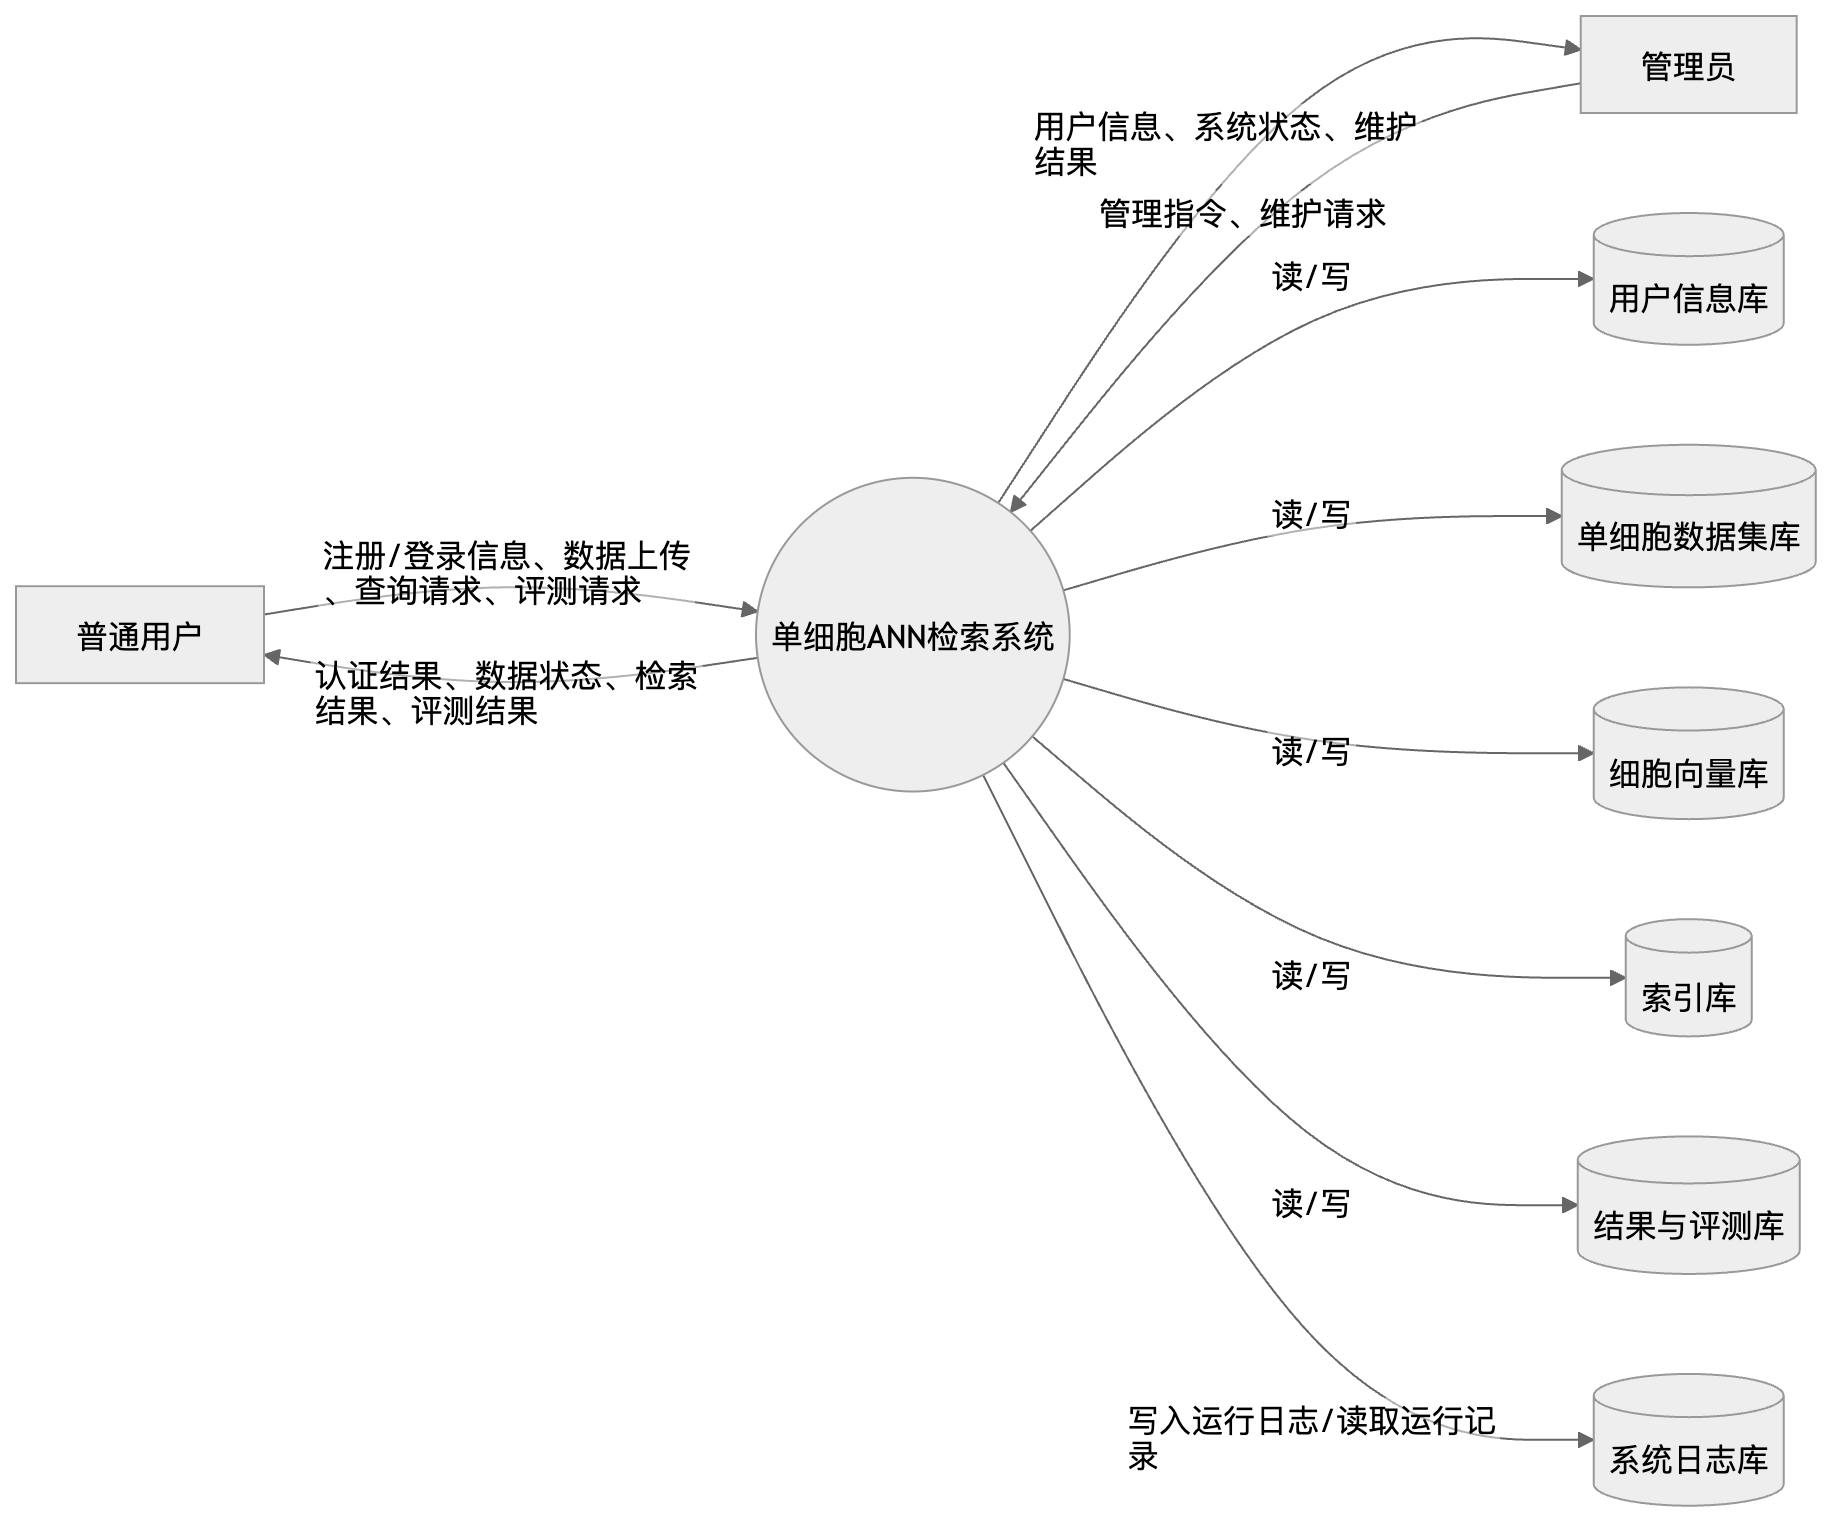
\includegraphics[width=0.95\textwidth]{system-top-level-data-flow.png}
  \caption{scANN 系统顶层数据流}
  \label{fig:top-data-flow}
\end{figure}

图\ref{fig:top-data-flow}展示了普通用户、管理员、核心处理过程与逻辑数据存储之间的关系。物理实现中，“向量库”对应经校验后从数据文件加载的连续 \code{float32} 矩阵，“索引库”对应索引文件及 JSON 清单，“结果与评测库”对应查询摘要和评测快照，而不是保存每一条 Top-K 结果。

\subsection{详细模块设计}

\paragraph{用户与权限。}注册时保存密码摘要；登录后签发带登录版本的 JWT。每次业务请求重新查询当前用户并校验版本，账号删除或密码变化后旧令牌失效。普通用户可使用检索功能，管理员额外拥有用户、非活动数据集和非活动索引的删除权限。

\paragraph{数据管理。}上传文件先写入临时位置，只有在格式、二维形状、非空、有限数和元信息行数全部通过后才原子发布。H5AD 默认读取 \code{obsm["X\_pca"]}，字段不存在时仅对默认配置回退到 \code{X}。系统对源文件、表示字段、向量内容和细胞顺序计算语义 SHA-256 指纹。

\paragraph{索引管理。}所有索引实现统一的构建、搜索、保存、加载、参数和序列化大小接口。索引清单绑定数据集 ID、语义指纹、维度、规模、算法、度量、参数、库版本和文件指纹；加载时逐项校验，失败不会污染当前索引。

\paragraph{检索与条件保证。}普通查询直接在活动索引中检索。条件查询不是对一次 ANN 结果简单后过滤，而是先确定满足 \code{cell\_type} 的候选集合，再在子集上做精确搜索。因此最坏情况下仍保证：每个返回项满足条件，数量为 $\min(K,n_f)$，且结果是条件候选集内的精确 Top-K，其中 $n_f$ 为条件候选数。

\paragraph{评测与可视化。}评测使用固定随机种子从同一数据集中无放回选取查询，以 Flat 结果作为 ground truth。查询结果通过表格、距离/得分条形图、类型分布和 UMAP/PCA 散点图展示；点击散点可回填细胞编号并触发新查询。

\paragraph{扩展服务。}联合检索在用户显式确认共享向量空间后拼接多数据集快照，并保存全局 ID 到“数据集+本地 ID”的来源映射。RAG 助手将自然语言限制为相似细胞、类型代表和数据集概览三类计划，再以真实检索证据和引用白名单约束回答。

\subsection{数据库设计}

\begin{table}[htbp]
  \centering
  \caption{主要数据库表}
  \label{tab:database}
  \begin{tabularx}{\textwidth}{p{0.19\textwidth}p{0.25\textwidth}Y}
    \toprule
    表名 & 用途 & 关键字段 \\
    \midrule
    \code{users} & 用户和角色 & username、password\_hash、role、created\_at \\
    \code{datasets} & 数据集元信息与活动状态 & name、stored\_path、format、n\_cells、dim、fingerprint、owner、active \\
    \code{index\_artifacts} & 持久化索引元信息 & dataset\_fingerprint、type、metric、parameters、paths、artifact\_fingerprint \\
    \code{query\_logs} & 查询摘要历史 & user、dataset、mode、cell\_id、K、index、metric、filters、query\_ms \\
    \code{evaluation\_logs} & 评测请求与结果快照 & user、dataset、K、query\_count、index\_types、results \\
    \bottomrule
  \end{tabularx}
\end{table}

数据库不保存上传文件内容、索引二进制、原始查询向量、RAG 问题或回答。文件路径以受控根目录内的相对路径保存，文档和接口响应不暴露开发机器目录。

\subsection{UI 设计}

UI 采用单页纵向工作台，将认证、数据集、索引持久化、联合检索、RAG、查询、评测和历史按业务依赖顺序排列。主要操作使用明确按钮和独立加载状态，错误区域具有 alert 语义，宽表格在窄屏下允许横向滚动。

\begin{figure}[htbp]
  \centering
  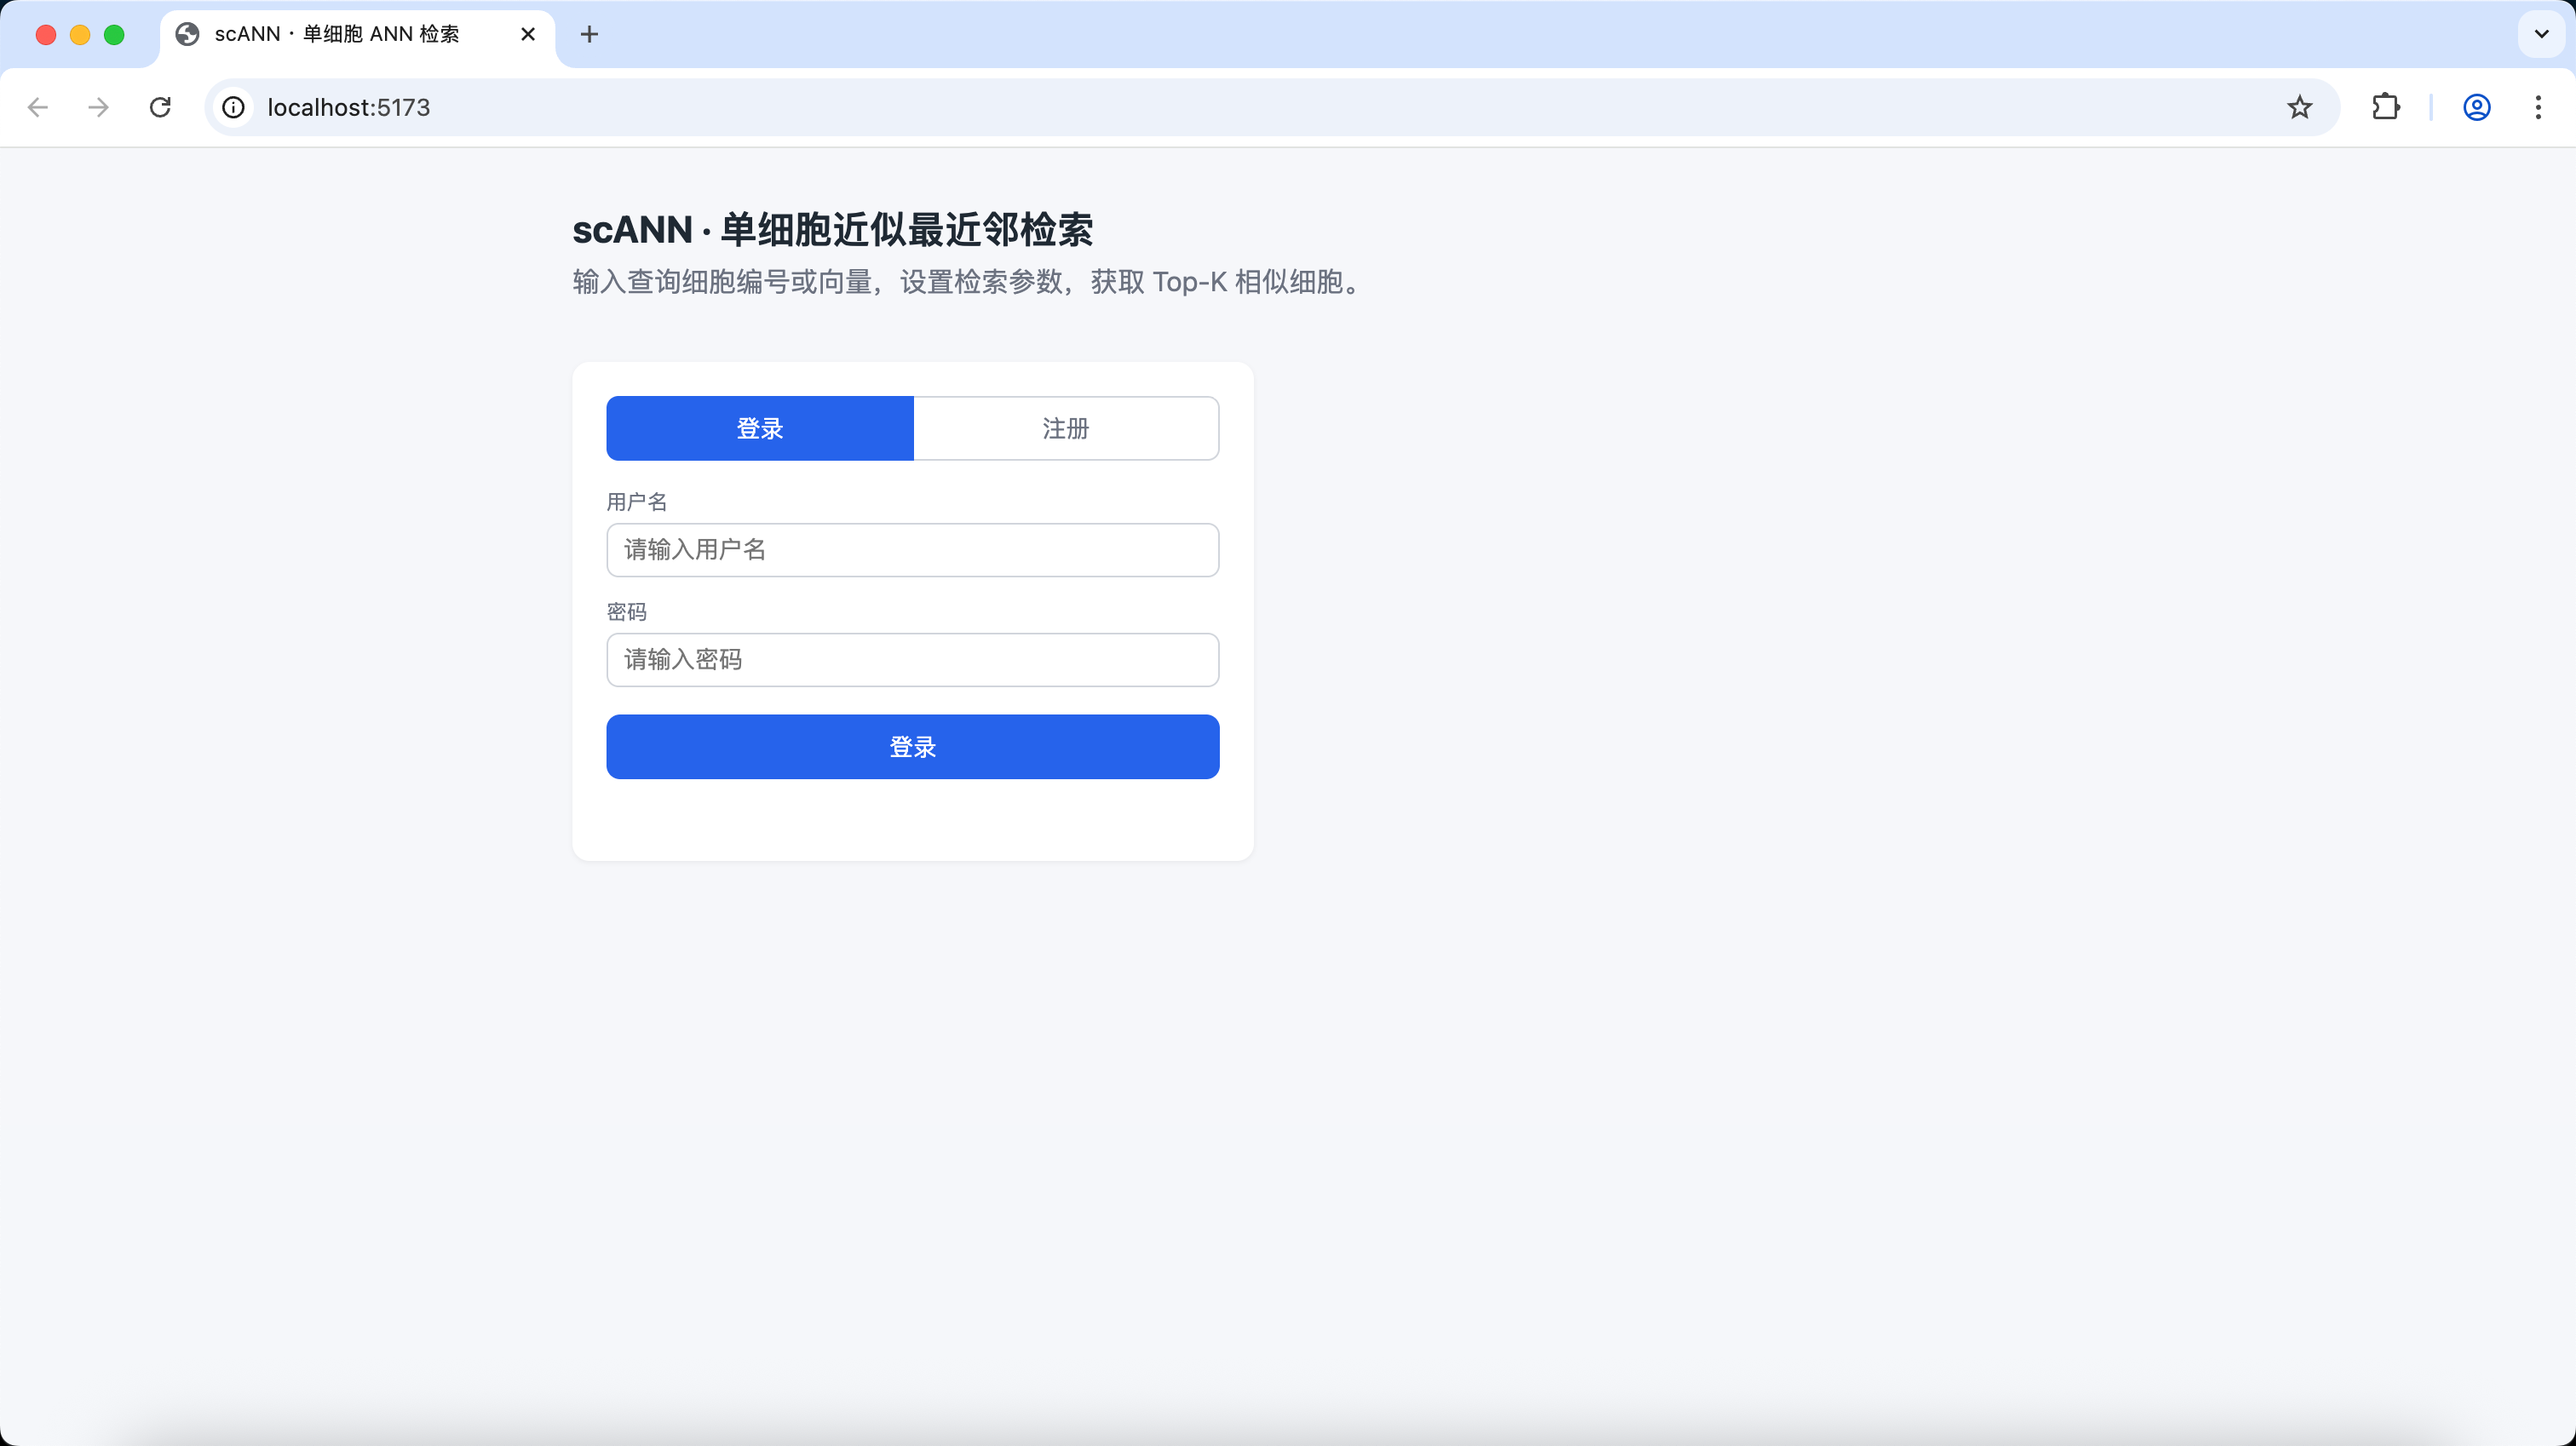
\includegraphics[width=0.86\textwidth]{04_login_panel.png}
  \caption{scANN 登录与注册入口}
  \label{fig:login}
\end{figure}

\begin{figure}[htbp]
  \centering
  \begin{subfigure}[t]{0.49\textwidth}
    \centering
    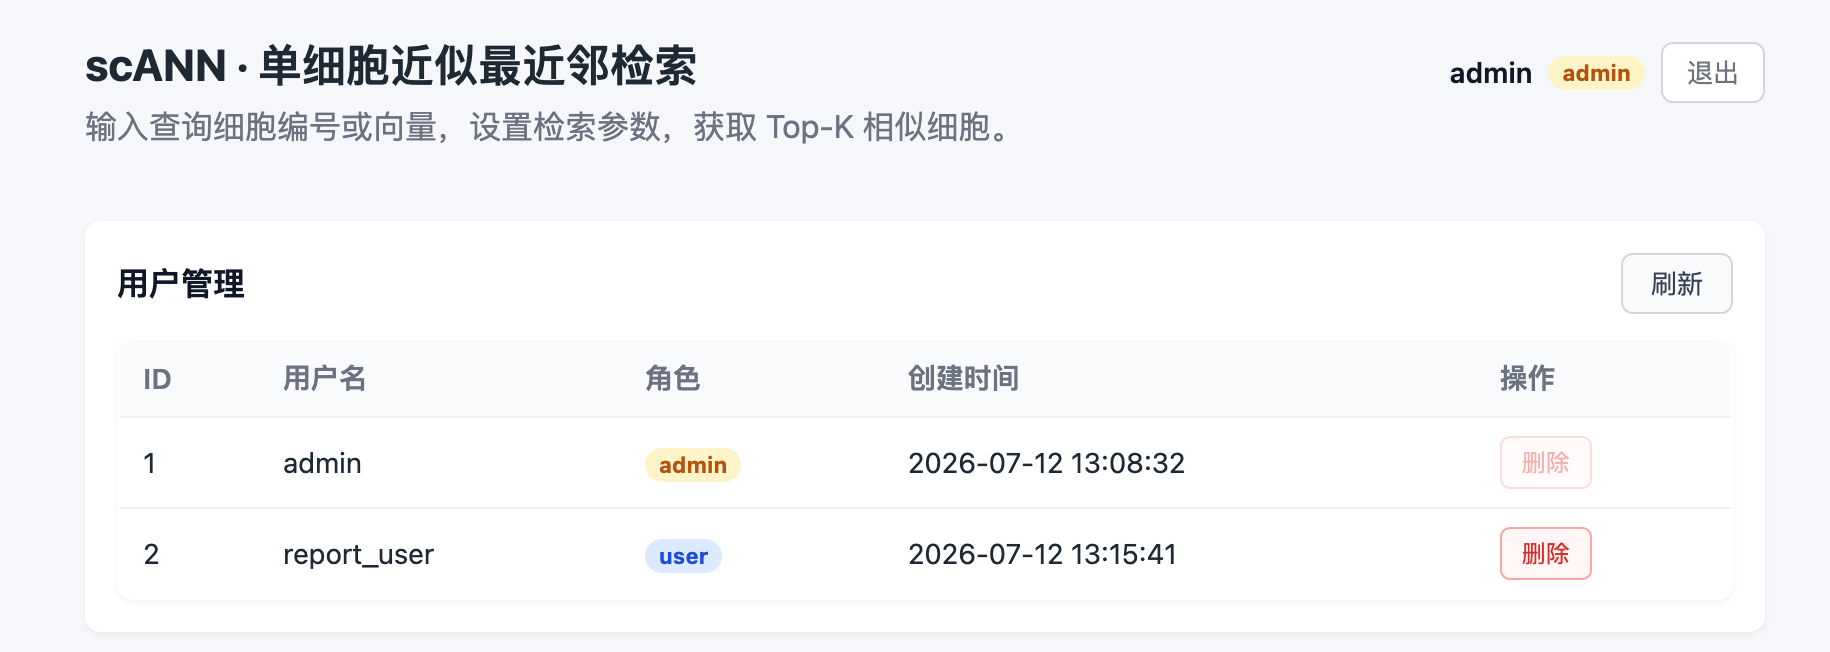
\includegraphics[width=\textwidth]{06_user_register_success.png}
    \caption{管理员用户列表与角色信息}
  \end{subfigure}
  \hfill
  \begin{subfigure}[t]{0.49\textwidth}
    \centering
    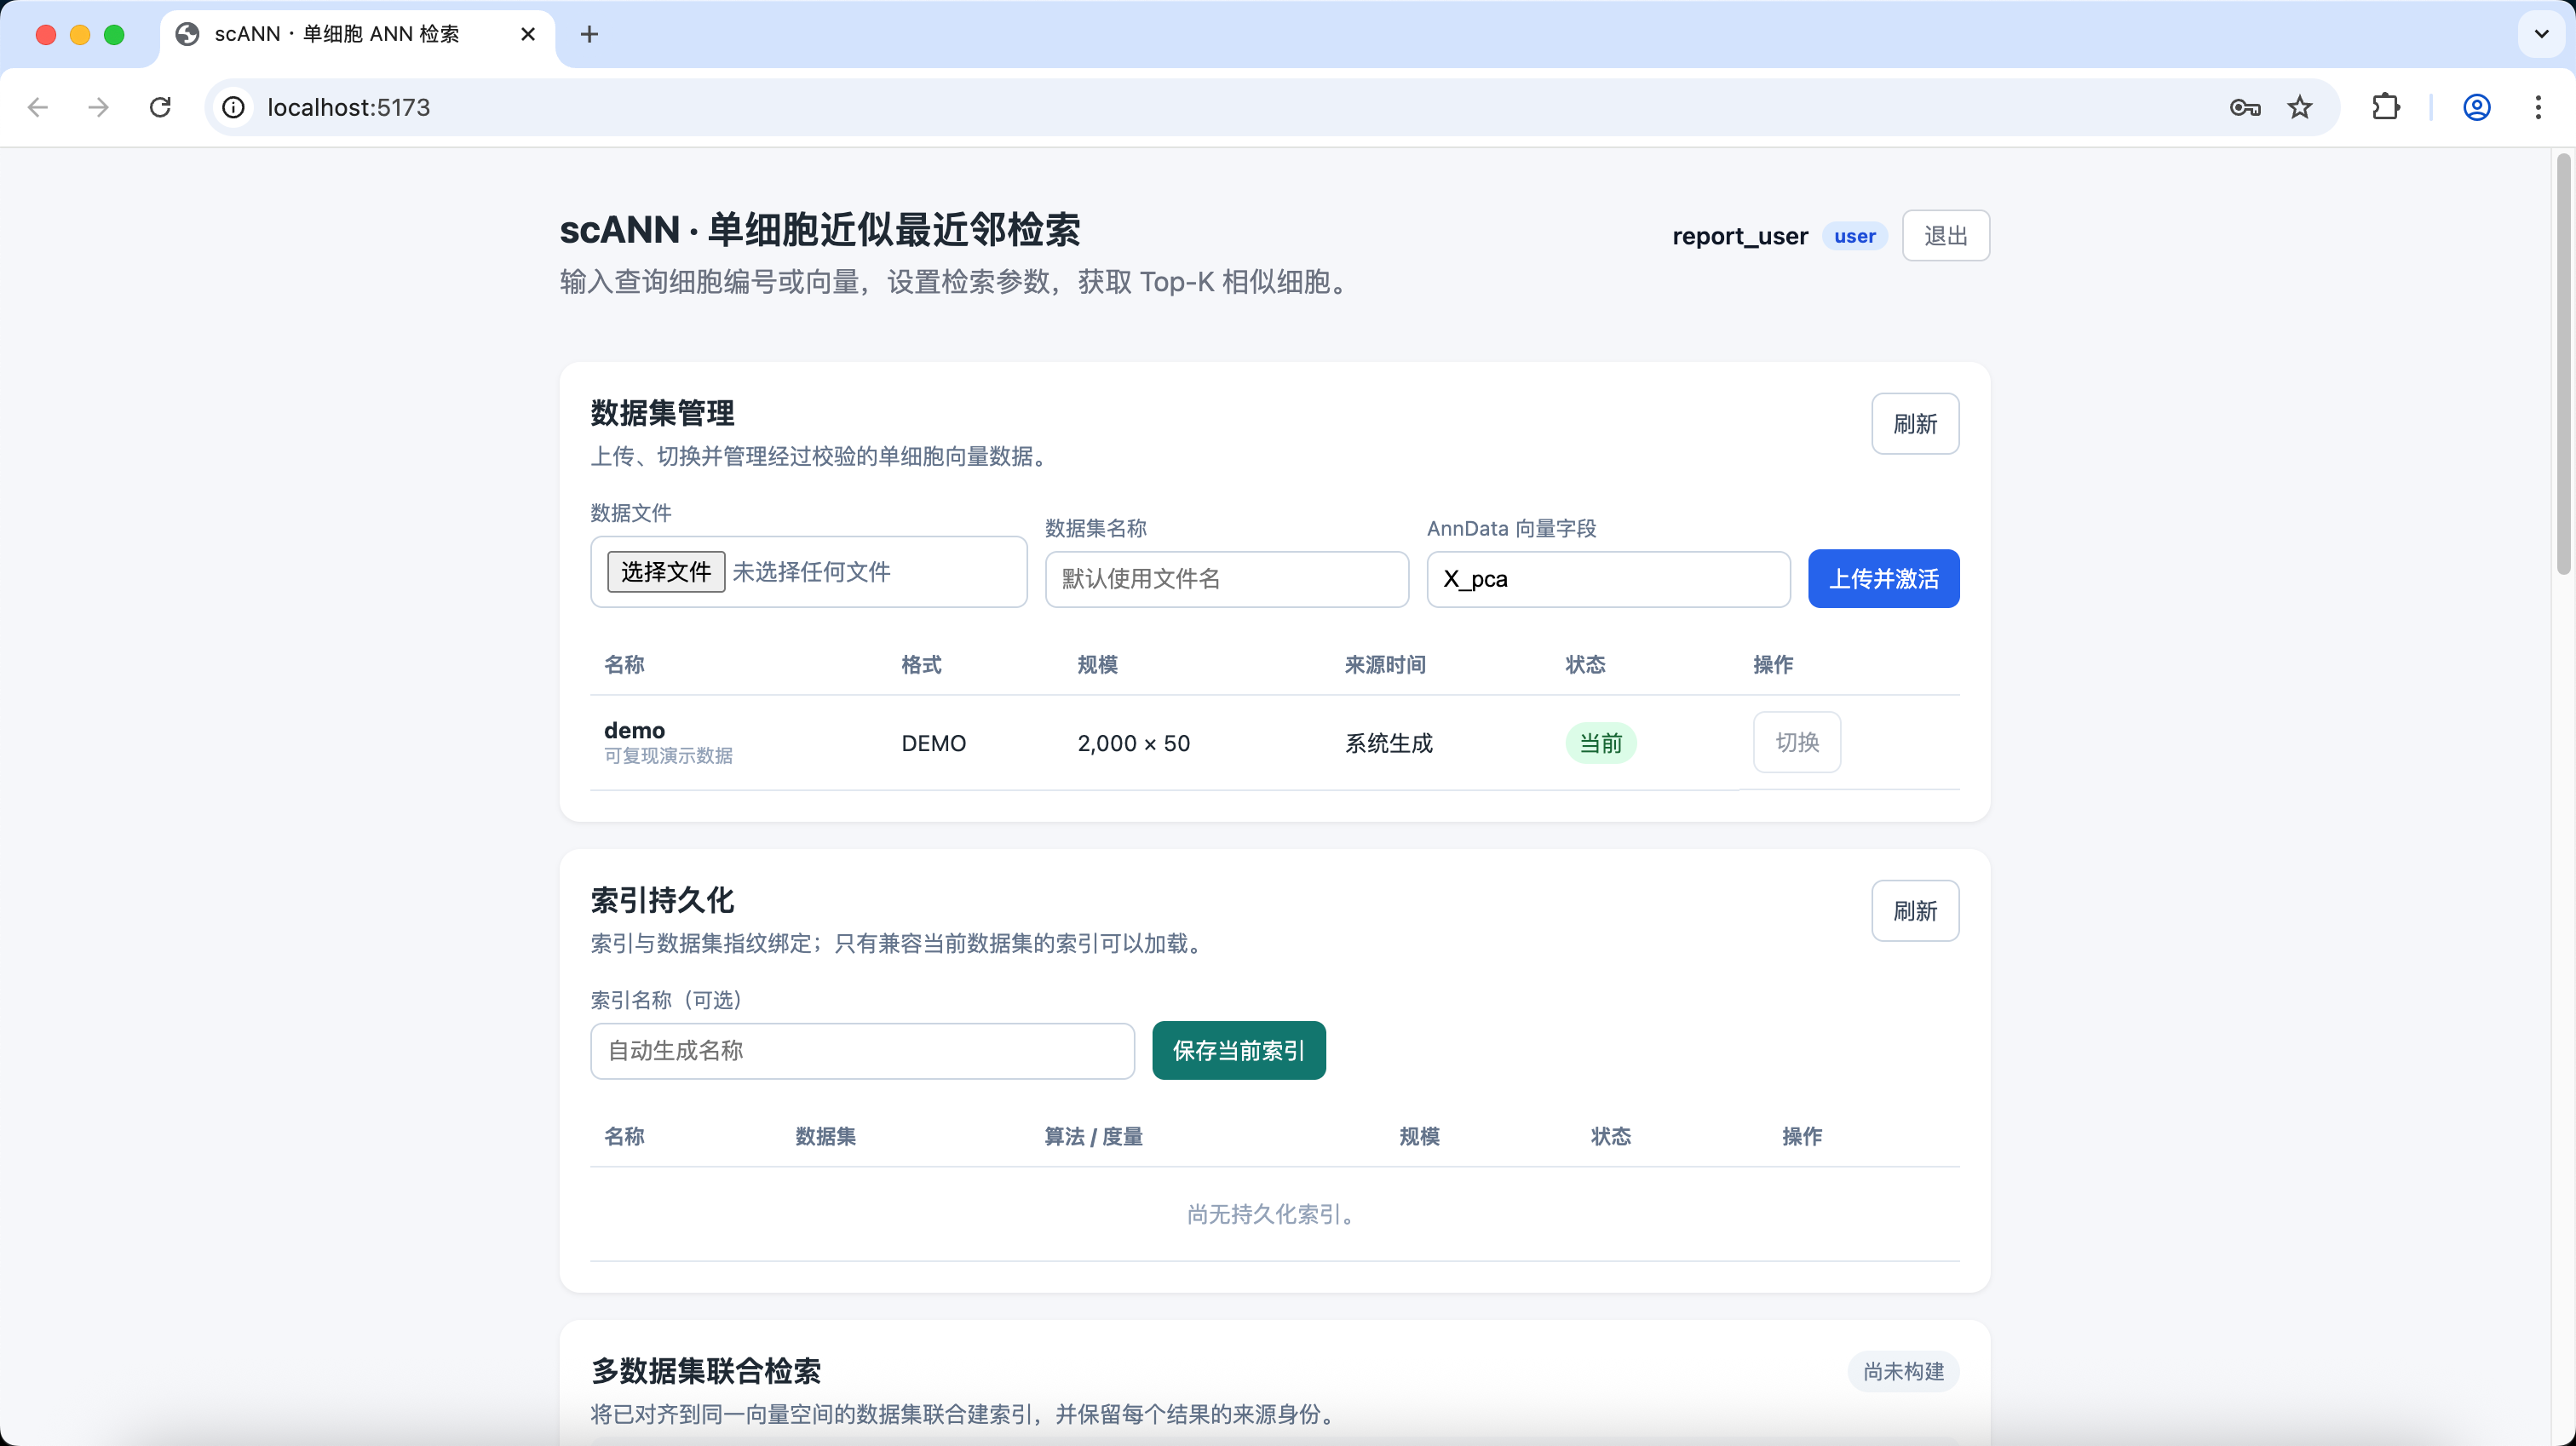
\includegraphics[width=\textwidth]{07_user_workspace_no_admin_controls.png}
    \caption{普通用户工作台无管理员控件}
  \end{subfigure}
  \caption{用户角色与权限隔离的界面验证}
  \label{fig:roles}
\end{figure}

\FloatBarrier
\section{数据与算法原理}

\subsection{AnnData 与实验数据}

AnnData 将主矩阵 \code{X}、细胞元信息 \code{obs}、特征元信息 \code{var}、多维表示 \code{obsm} 和分层数据 \code{layers} 组织在同一带注释矩阵中\cite{anndata}。本系统读取两个 H5AD 文件，实际用于检索的是 30 维 \code{X\_pca}，而不是 32,397 维原始表达矩阵。

\begin{table}[htbp]
  \centering
  \caption{真实 H5AD 数据统计}
  \label{tab:datasets}
  \begin{tabularx}{\textwidth}{p{0.24\textwidth}p{0.16\textwidth}p{0.16\textwidth}p{0.15\textwidth}Y}
    \toprule
    数据集 & 细胞数 & 原始特征数 & 检索维度 & 标题 \\
    \midrule
    \code{liver-main} & 69,032 & 32,397 & 30 & 健康儿童与成人肝组织 \\
    \code{liver-ifald-supplement} & 81,001 & 32,397 & 30 & 健康与 IFALD 儿童及成人肝组织 \\
    \bottomrule
  \end{tabularx}
\end{table}

两个文件内嵌的 \code{uns["citation"]} 均指向同一研究论文 DOI 和 CZ CELLxGENE collection\cite{liverpaper,cellxgene}。许可证信息未在仓库中得到可靠确认，正式对外发布前仍需项目组核对原始集合的许可与引用要求。

系统的“预处理”边界是：选择表示、转换连续 \code{float32}、校验二维形状、样本数、有限数和元信息行数。系统没有重新执行原始测序 QC、归一化、对数变换、高变基因筛选或 PCA 训练，因此实验结果应解释为“对已有表征的向量检索”，而不是完整单细胞分析流程。

\begin{figure}[htbp]
  \centering
  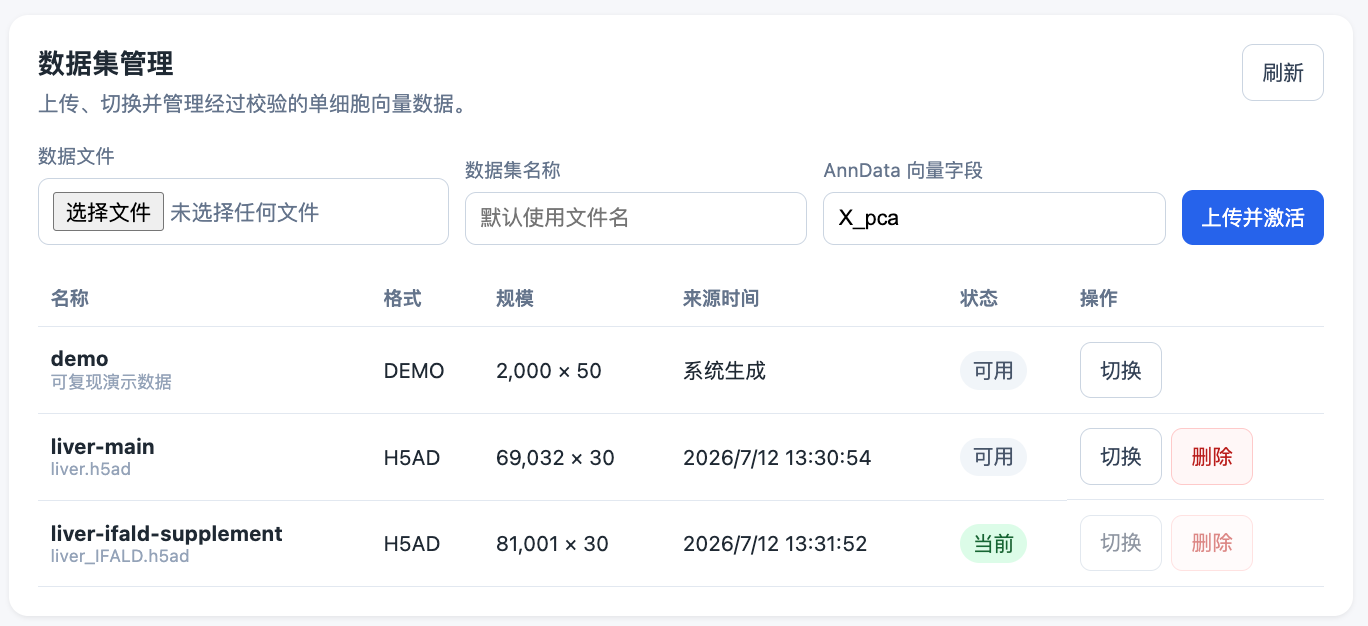
\includegraphics[width=0.82\textwidth]{17_upload_liver_ifald.png}
  \caption{主数据集与补充 H5AD 的导入和管理}
  \label{fig:dataset-management}
\end{figure}

\subsection{距离度量}

对于查询向量 $q$ 与候选向量 $x$，系统支持：

\begin{align}
d_{L2}(q,x) &= \sum_{j=1}^{d}(q_j-x_j)^2,\\
d_{cos}(q,x) &= 1-\frac{q^\top x}{\lVert q\rVert_2\lVert x\rVert_2},\\
s_{IP}(q,x) &= q^\top x.
\end{align}

平方 L2 与 Cosine 距离越小越相似，内积得分越大越相似。Cosine 索引在构建和查询前对向量归一化，保证 FAISS 内积与余弦相似度一致。

\subsection{索引方法}

\paragraph{Flat。}Flat 对全部向量计算精确距离，召回率为 1，是评测 ground truth；其时间复杂度随细胞数和维度线性增长。

\paragraph{IVF。}IVF 使用聚类中心划分倒排单元，查询时只扫描若干最接近的单元。\code{nlist} 与 \code{nprobe} 控制构建、速度和召回之间的权衡\cite{faisswiki}。

\paragraph{HNSW。}HNSW 构建多层近邻图，从稀疏上层快速导航到局部密集区域，\code{M}、\code{efConstruction} 和 \code{efSearch} 分别影响图连接、构建质量和查询搜索宽度\cite{hnsw}。

\paragraph{PQ。}乘积量化把向量拆为多个子向量并分别量化，以短编码近似原向量，从而显著减少索引存储，但压缩域距离会带来排序误差\cite{pq,faisswiki}。

\subsection{PQ 候选精确重排及最坏情况保证}

改进版与基础 PQ 使用同一索引和码本。查询时先从 PQ 取出 $rK$ 个候选，本项目取 $r=4$，再用已加载的原始向量计算真实距离并返回前 K。设精确 Top-K 为 $G$，基础 PQ Top-K 为 $P$，扩大候选集为 $C$，精确重排结果为 $R$。因为 $P\subseteq C$，且精确排序会优先选择 $C\cap G$，有

\begin{equation}
|R\cap G|=\min(K,|C\cap G|)\geq |P\cap G|.
\end{equation}

因此在无歧义的精确距离全序和相同 PQ 候选序列下，重排 Recall@K 不低于基础 PQ。该保证的下界是基础 PQ Recall，上界是 $|C\cap G|/K$：若真实近邻没有进入 $C$，重排也无法恢复。扩大 $r$ 会提高候选覆盖概率，同时增加精确计算成本；当 $C$ 覆盖全部数据时则退化为精确扫描。

\section{系统实现与功能实验}

\subsection{索引构建与持久化}

图\ref{fig:hnsw-build}显示 demo 数据上成功构建 HNSW/Cosine 索引，页面同时展示数据规模、向量维度、度量、索引状态和构建耗时。图\ref{fig:index-save}展示真实数据集上的 HNSW 索引持久化记录。现有截图只证明“保存成功”，索引加载由自动化测试验证，不把缺失的加载截图写成界面证据。

\begin{figure}[htbp]
  \centering
  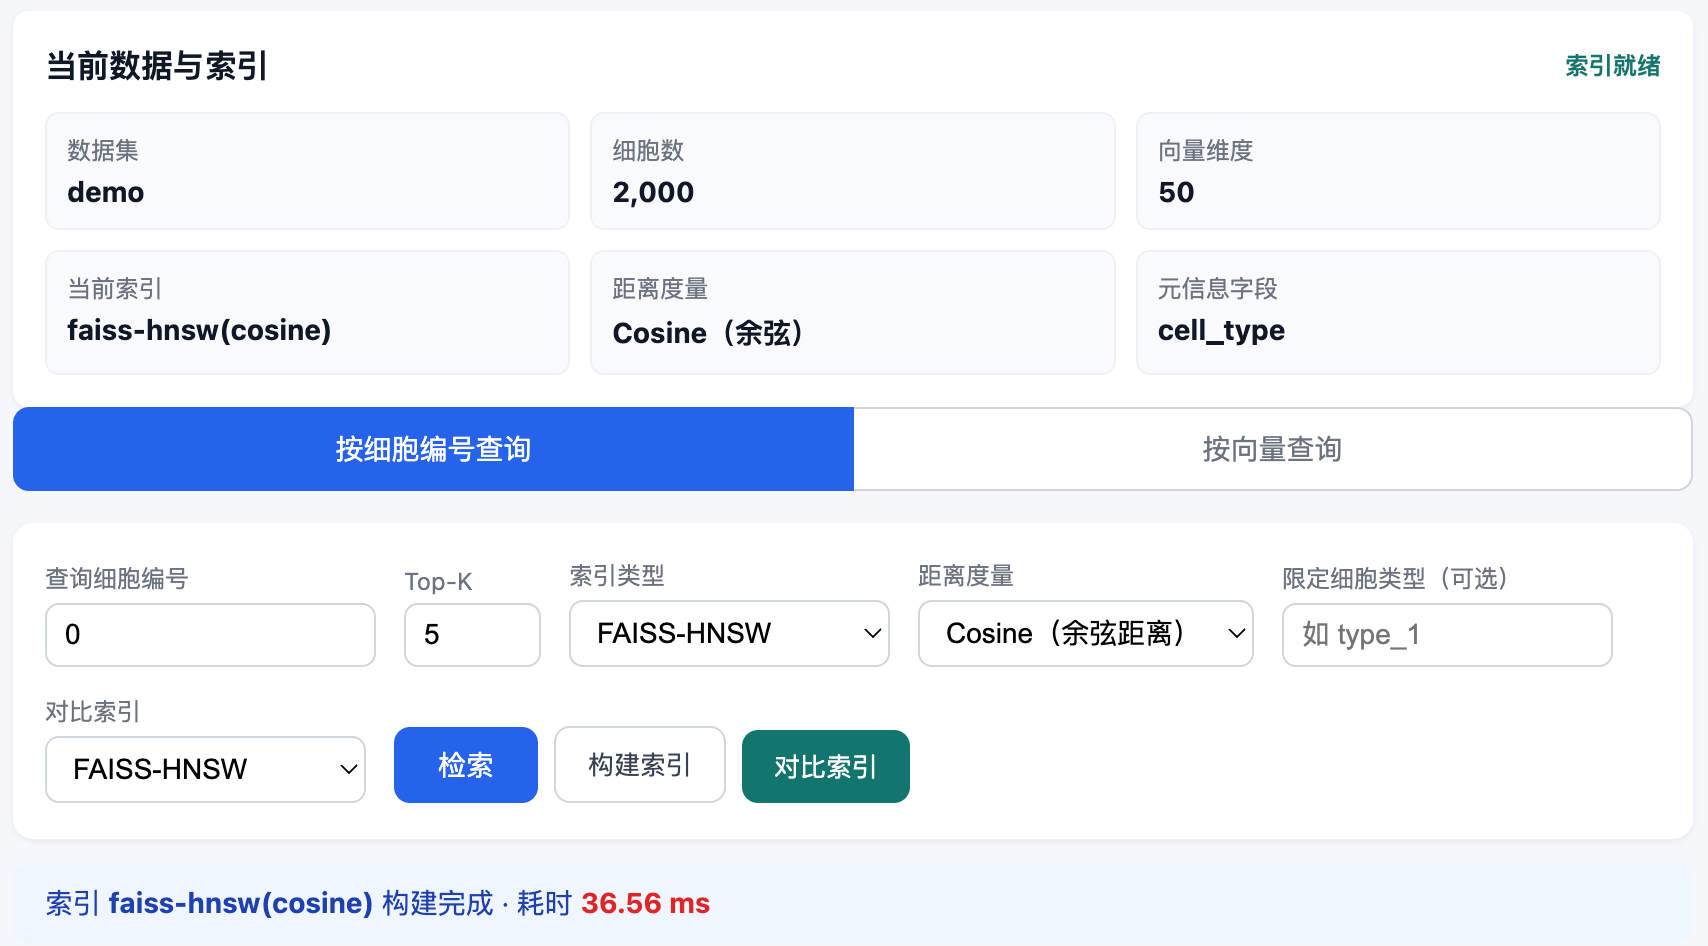
\includegraphics[width=0.82\textwidth]{09_hnsw_index_built.png}
  \caption{HNSW 索引构建及运行状态}
  \label{fig:hnsw-build}
\end{figure}

\begin{figure}[htbp]
  \centering
  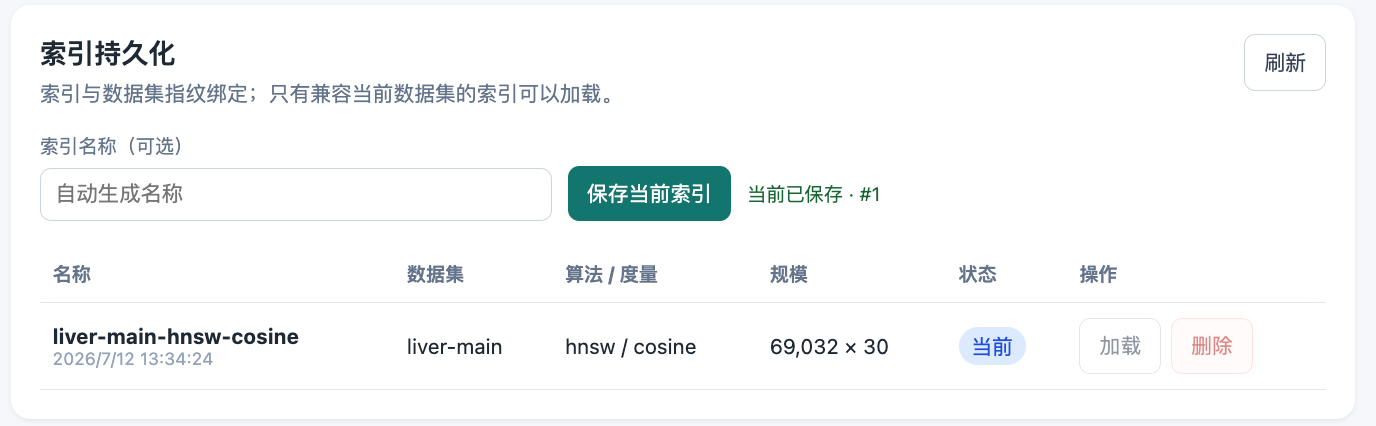
\includegraphics[width=0.78\textwidth]{20_index_saved.png}
  \caption{HNSW 索引持久化记录}
  \label{fig:index-save}
\end{figure}

\subsection{细胞查询、向量查询与条件检索}

按细胞编号查询会自动排除查询细胞自身；按向量查询要求逗号分隔的有限数值数量与当前维度相同。图\ref{fig:cell-search}在 demo 数据上展示 Top-5 结果、余弦距离、类型分布和结果表；图\ref{fig:real-search}展示真实 PCA 表征上的 L2 Top-5 结果。后者能证明真实数据检索结果，但画面未包含输入框，因此图注不将其夸大为“手工输入 30 维向量”的独立证据。

\begin{figure}[htbp]
  \centering
  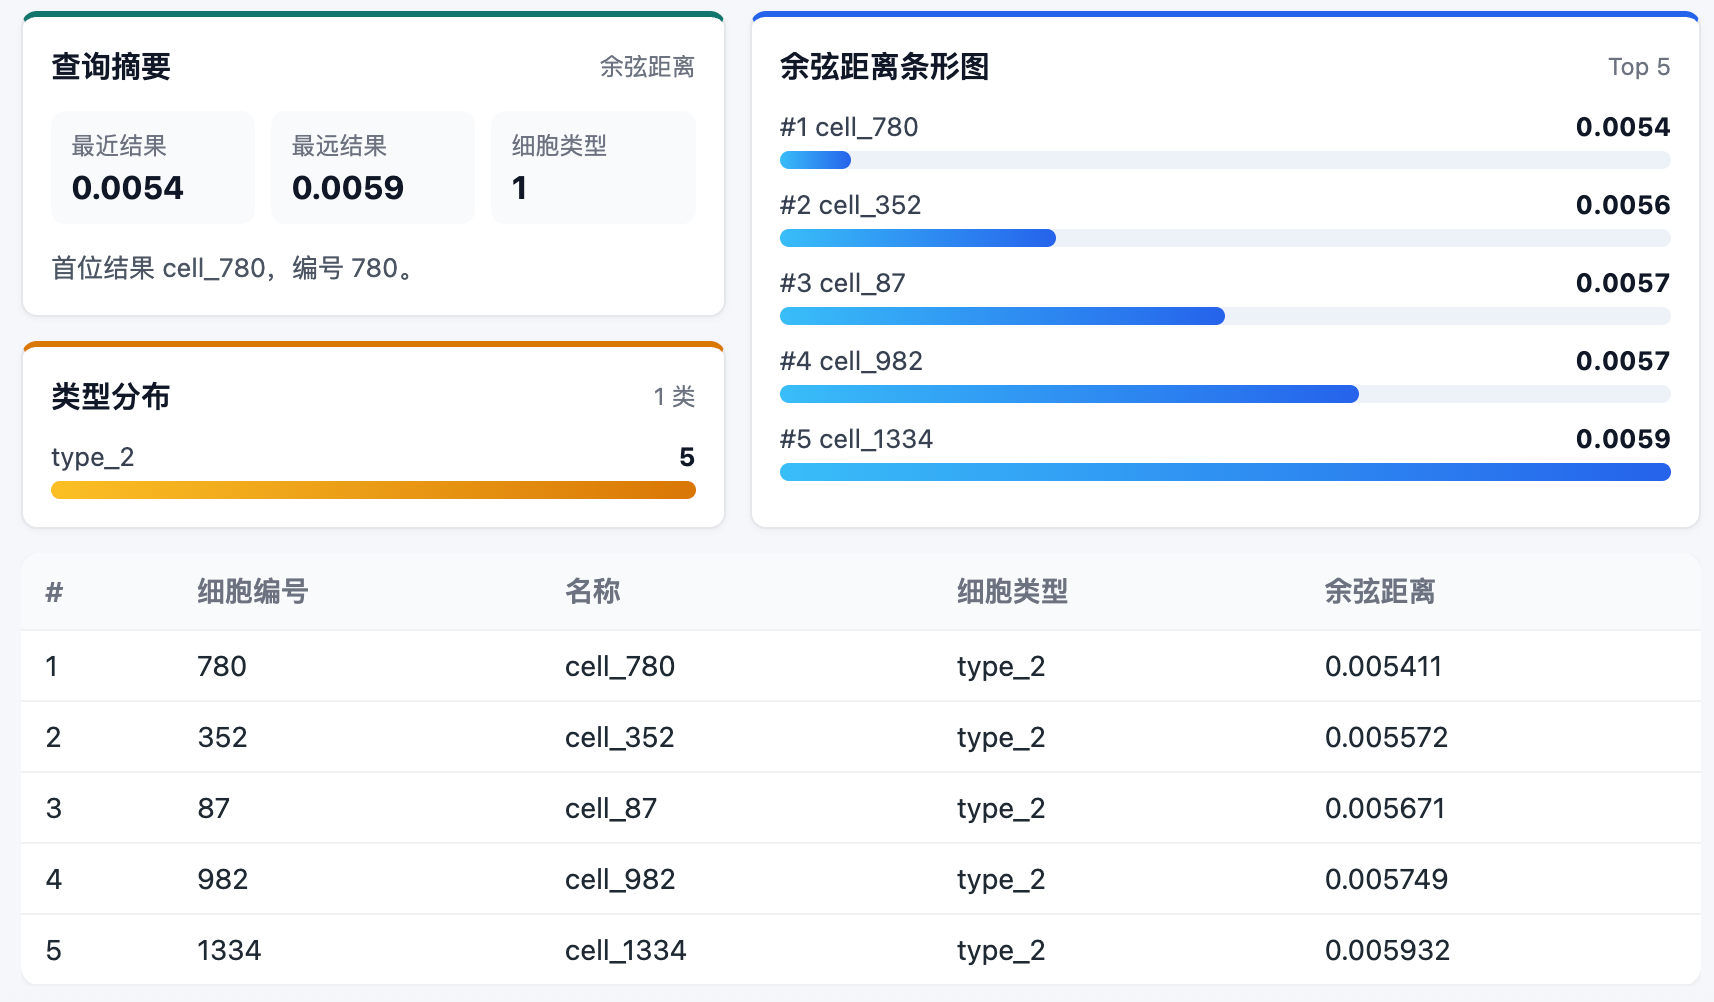
\includegraphics[width=0.90\textwidth]{10_cell_search_results.png}
  \caption{按细胞编号检索的 Top-5 结果及分布}
  \label{fig:cell-search}
\end{figure}

\begin{figure}[htbp]
  \centering
  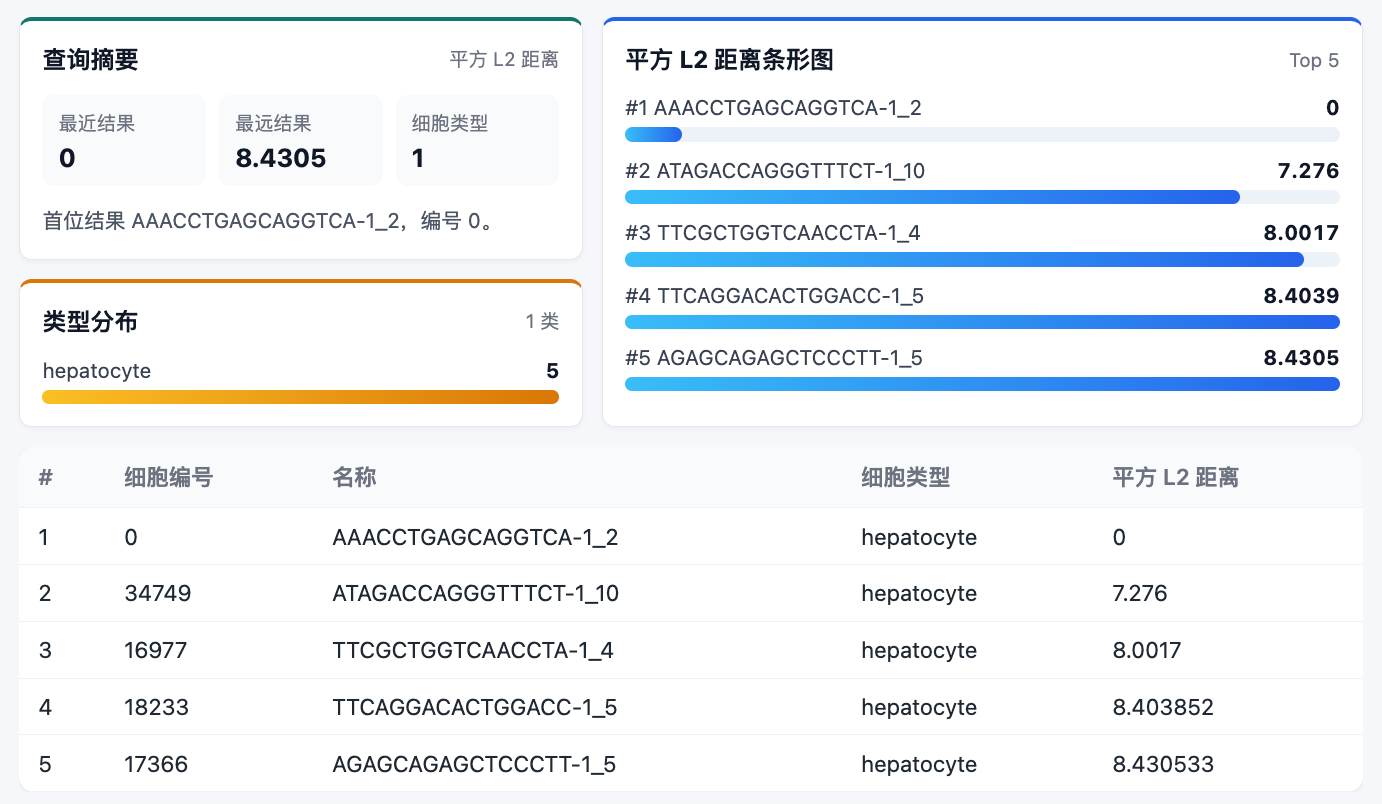
\includegraphics[width=0.87\textwidth]{19_vector_search_results.png}
  \caption{真实 PCA 表征上的 Top-5 相似细胞结果}
  \label{fig:real-search}
\end{figure}

条件检索当前只支持 \code{cell\_type}。自动化测试覆盖候选数多于 K、少于 K、空候选和不同度量，验证所有返回项满足条件且结果为条件子集内精确 Top-K。截图 \code{12} 与图\ref{fig:cell-search}画面重复且没有显示条件输入，因此未收入报告。

\subsection{二维可视化与图上查询}

UMAP 将高维流形映射到二维，适合交互式观察局部结构，但二维距离不应替代原始表示上的检索距离\cite{umap}。系统采用确定性抽样，并强制补入查询细胞与 Top-K 结果；红色表示查询细胞，蓝色表示近邻，背景点按类型着色。图\ref{fig:embedding}展示结果高亮，图\ref{fig:plot-query}展示选择新点后刷新查询结果的状态。

\begin{figure}[htbp]
  \centering
  \begin{subfigure}[t]{0.48\textwidth}
    \centering
    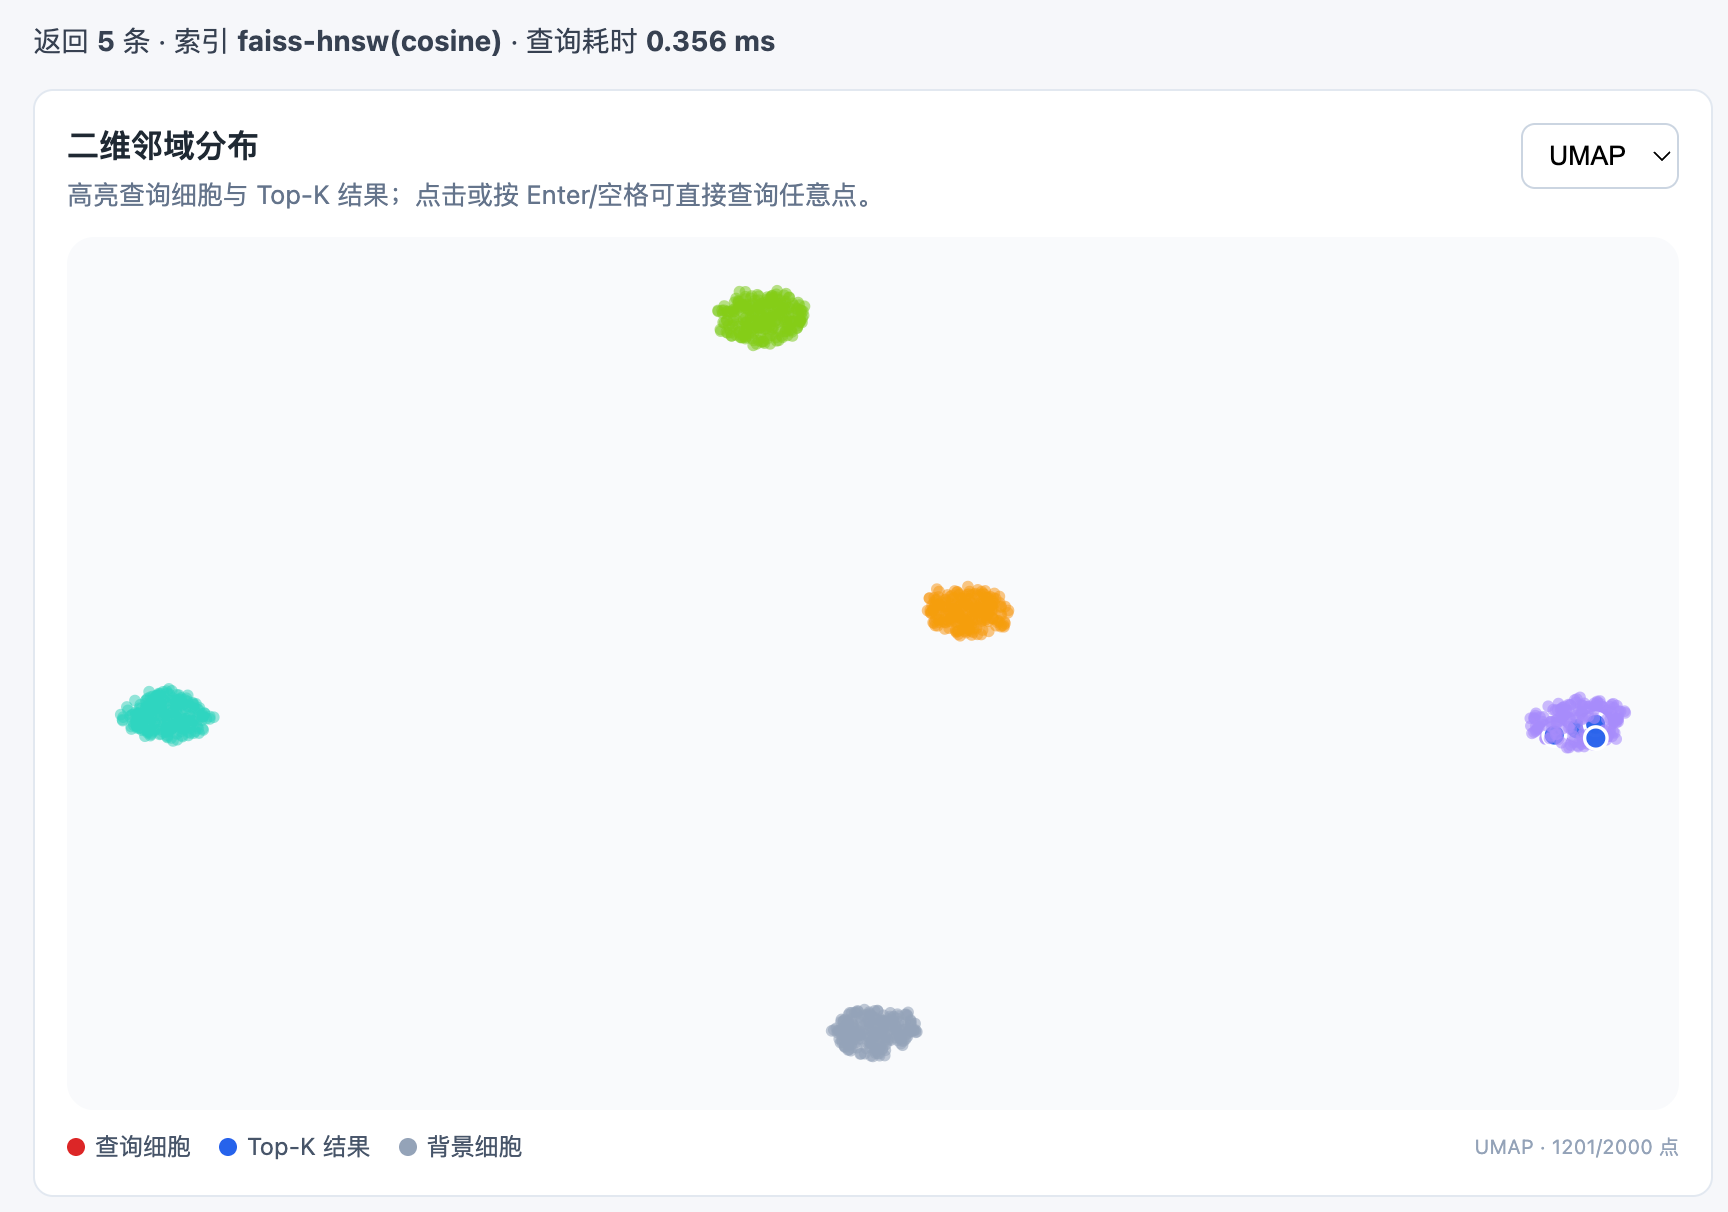
\includegraphics[width=\textwidth]{14_embedding_plot_highlight.png}
    \caption{查询细胞与近邻高亮}
    \label{fig:embedding}
  \end{subfigure}
  \hfill
  \begin{subfigure}[t]{0.48\textwidth}
    \centering
    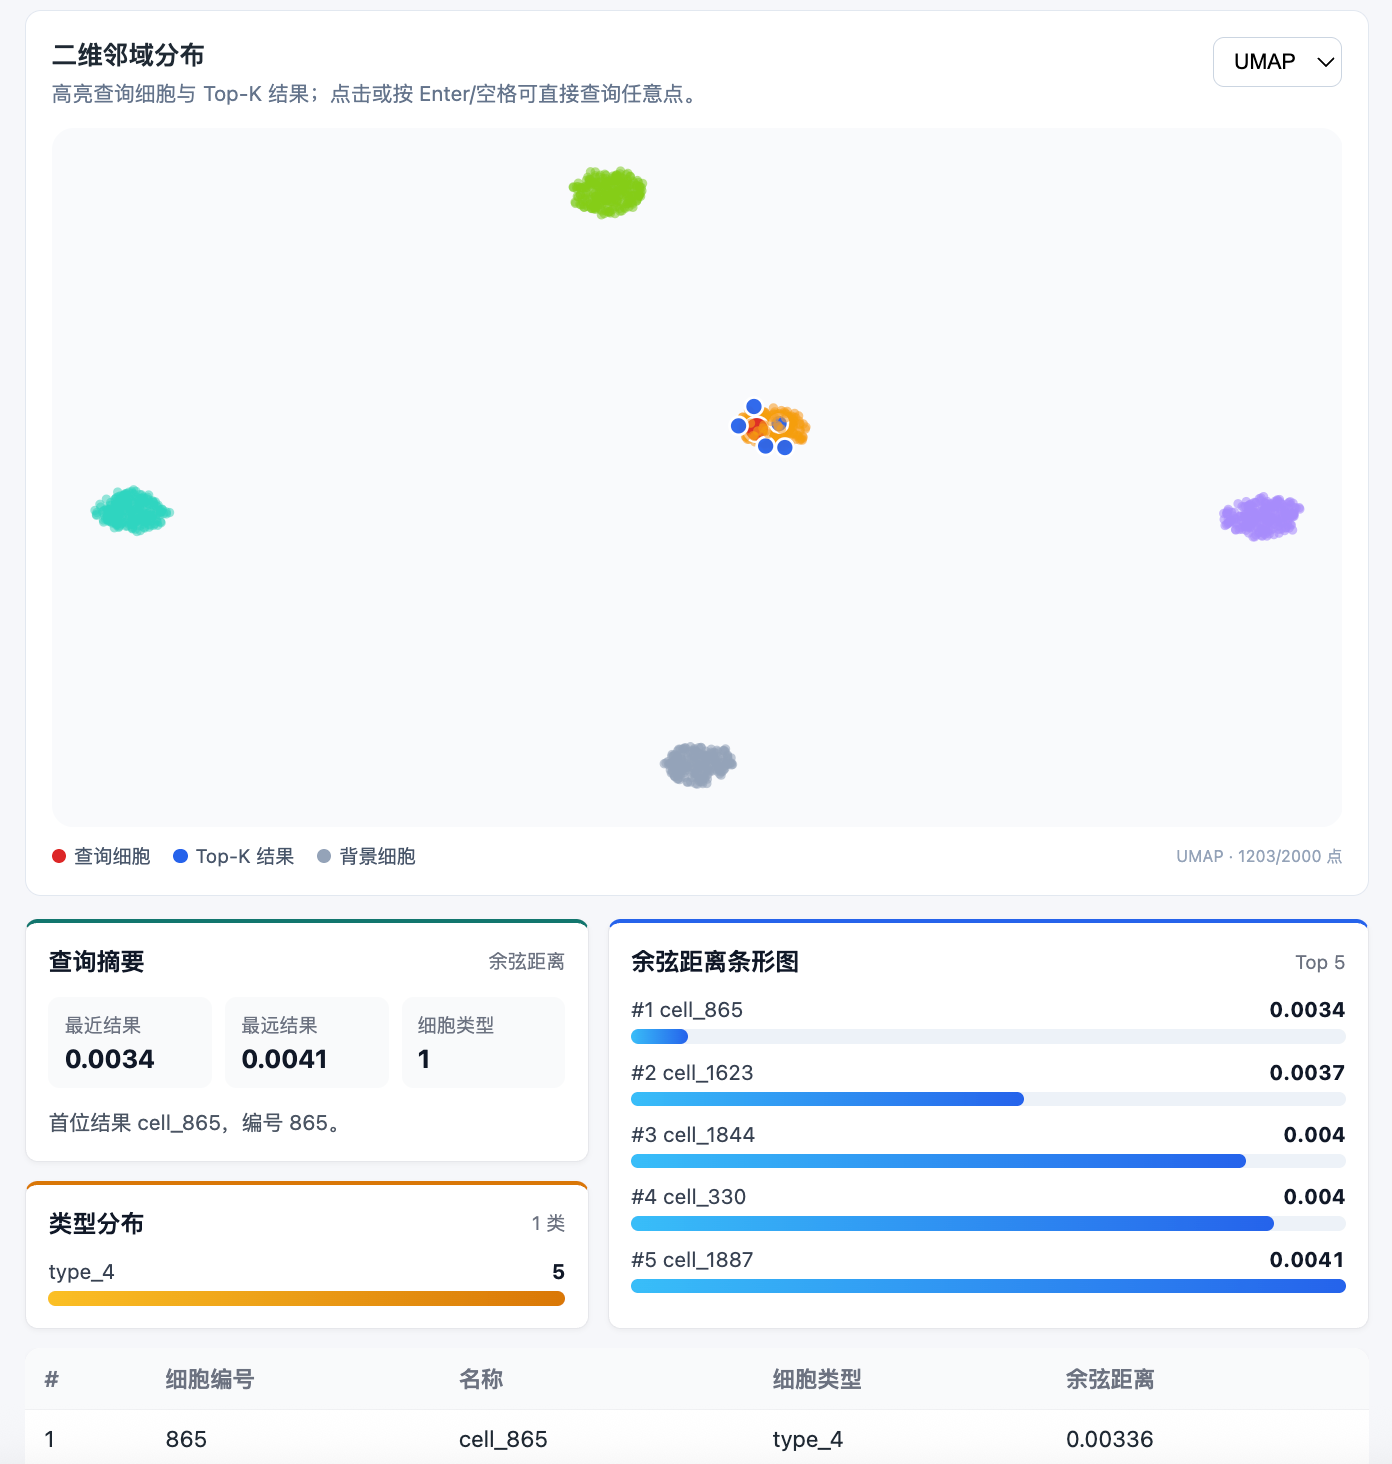
\includegraphics[width=0.78\textwidth]{15_plot_driven_query.png}
    \caption{图上选点后的新一轮查询}
    \label{fig:plot-query}
  \end{subfigure}
  \caption{UMAP 交互式邻域可视化}
\end{figure}

\subsection{运行历史}

查询历史记录用户、数据集、查询模式、索引、度量、Top-K、返回数和索引调用耗时，但向量查询不保存原始向量。普通用户只读取自己的记录，管理员可查看全局摘要。图\ref{fig:history}展示了多种查询模式和索引的历史记录。

\begin{figure}[htbp]
  \centering
  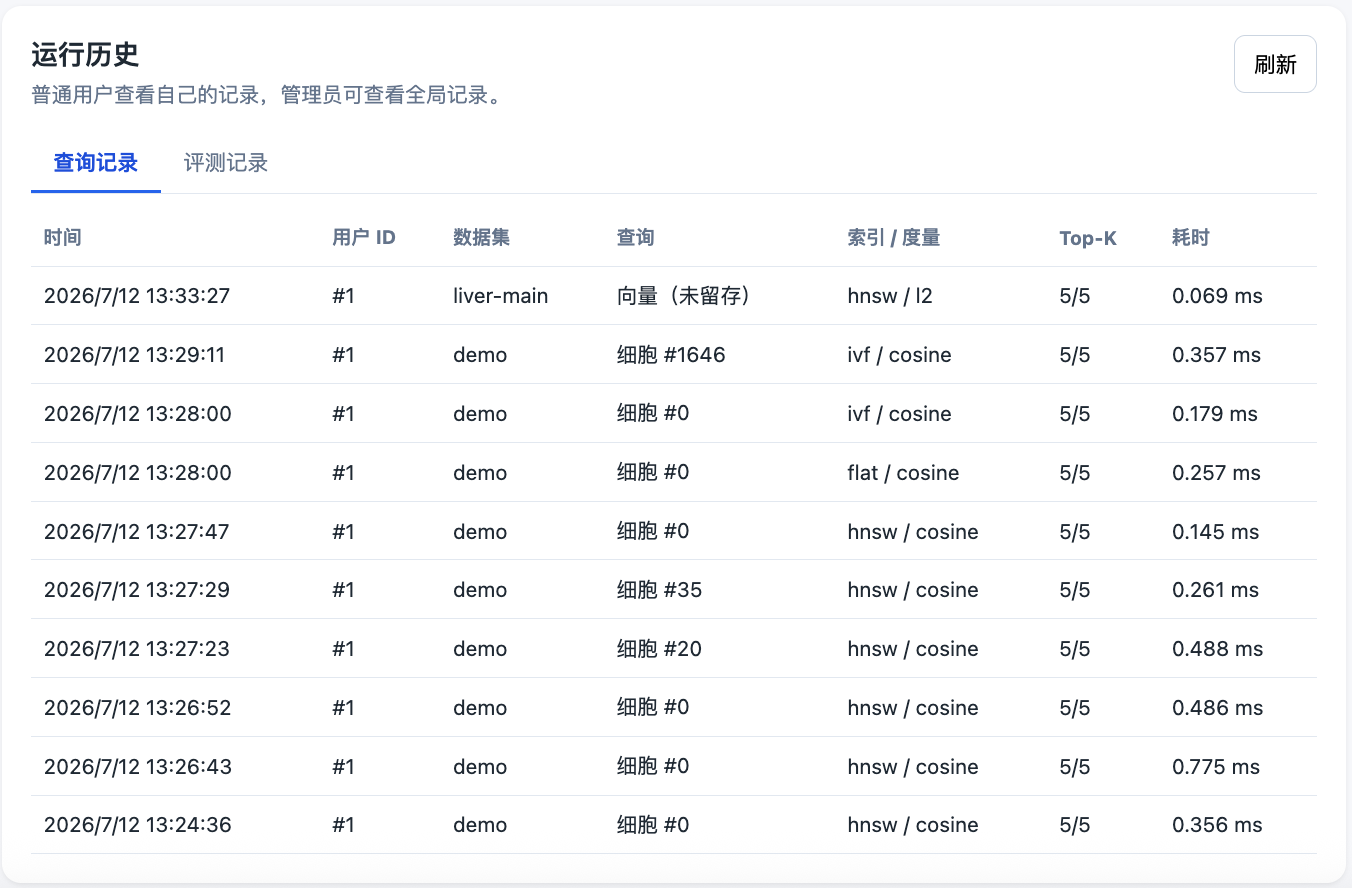
\includegraphics[width=0.86\textwidth]{29_query_history.png}
  \caption{查询运行历史及耗时记录}
  \label{fig:history}
\end{figure}

\FloatBarrier
\section{性能实验与结果分析}

\subsection{实验口径与指标}

主实验数据为 \code{liver-main} 的 69,032 个 30 维 \code{X\_pca} 向量。截图实验使用 L2、K=5、随机种子 42 和 12 个无放回查询；补充实验保持数据、度量和种子不变，将查询数提高到 200，并考察 K=1、5、10、20。各方法使用同一查询集合，以 Flat 为 ground truth，并在计算召回前排除查询细胞自身。

若第 $i$ 个查询的精确结果集合为 $G_i$，被测索引结果集合为 $A_i$，则

\begin{equation}
\mathrm{Recall@K}=\frac{1}{Q}\sum_{i=1}^{Q}\frac{|G_i\cap A_i|}{K}.
\end{equation}

平均查询耗时只包围索引 \code{search} 调用，不包含浏览器、HTTP、序列化、数据库历史写入和页面渲染。索引字节是稳定序列化结果，不等于进程峰值内存，也不包含原始数据矩阵。

\subsection{K=5 多索引对比}

\begin{figure}[htbp]
  \centering
  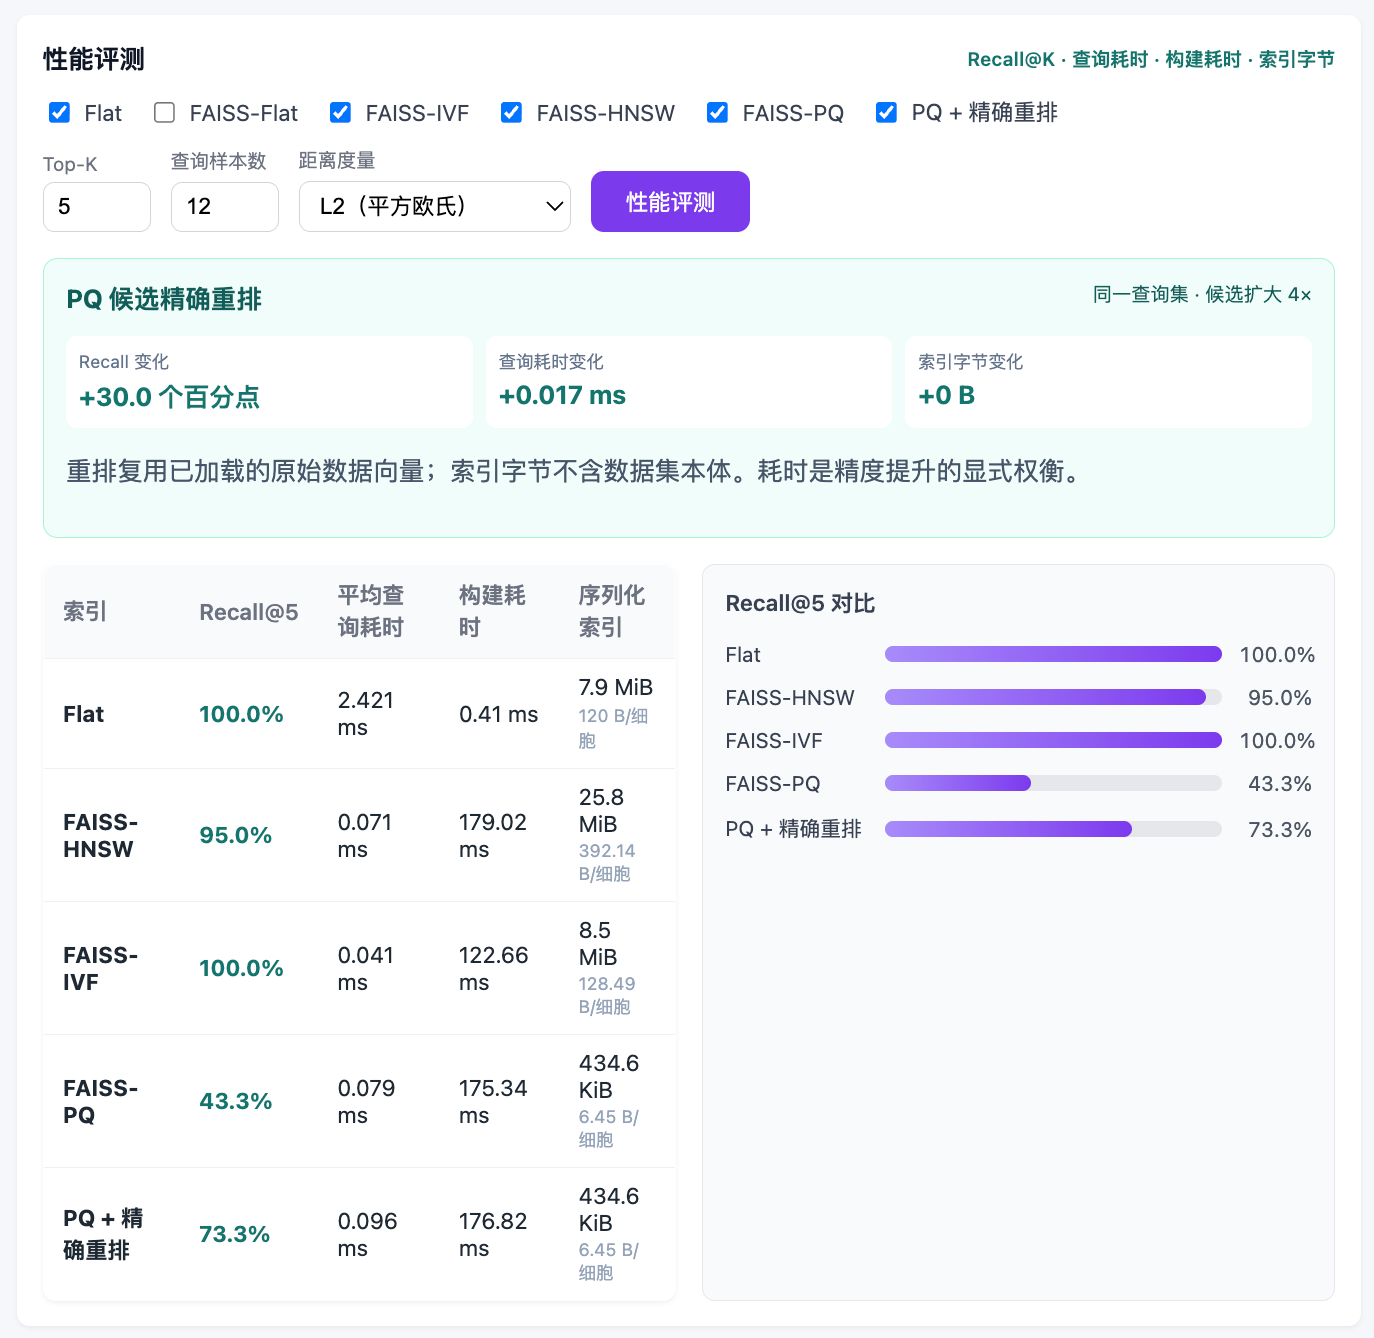
\includegraphics[width=0.76\textwidth]{22_eval_multi_index.png}
  \caption{不同索引方法的检索质量、效率与空间开销对比}
  \label{fig:evaluation}
\end{figure}

\begin{table}[htbp]
  \centering
  \caption{页面采集的 K=5、12 查询评测结果}
  \label{tab:k5-results}
  \begin{tabular}{lrrrr}
    \toprule
    索引 & Recall@5 & 平均查询/ms & 构建/ms & 序列化索引 \\
    \midrule
    Flat & 1.000 & 2.421 & 0.41 & 7.9 MiB \\
    FAISS-HNSW & 0.950 & 0.071 & 179.02 & 25.8 MiB \\
    FAISS-IVF & 1.000 & 0.041 & 122.66 & 8.5 MiB \\
    FAISS-PQ & 0.433 & 0.079 & 175.34 & 434.6 KiB \\
    PQ + 精确重排 & 0.733 & 0.096 & 176.82 & 434.6 KiB \\
    \bottomrule
  \end{tabular}
\end{table}

在该小样本演示中，IVF 相比 Flat 的索引调用平均耗时降低约 $2.421/0.041=59.0$ 倍，且 12 个查询上 Recall@5 为 1；HNSW 降低约 34.1 倍，但序列化索引约为 Flat 的 3.27 倍。PQ 索引只有 Flat 的约 5.37\%，即约缩小 18.6 倍，但 Recall@5 降至 0.433。该结果说明查询时间、构建成本、召回和空间必须联合分析，不能用单一指标判断“最佳索引”。

PQ 精确重排使用完全相同的 434.6 KiB PQ 索引，以 0.017 ms 的额外平均查询时间将 Recall@5 提高 0.300，即 30.0 个百分点。由于仅有 12 个查询，这一数值用于演示系统的成对评测能力，不作为跨机器或跨数据的稳定性能承诺。

\subsection{不同 Top-K 的补充实验}

\begin{table}[htbp]
  \centering
  \caption{200 个固定查询下的 Recall@K}
  \label{tab:multik-recall}
  \begin{tabular}{lrrrr}
    \toprule
    索引 & K=1 & K=5 & K=10 & K=20 \\
    \midrule
    Flat & 1.0000 & 1.0000 & 1.0000 & 1.0000 \\
    FAISS-IVF & 1.0000 & 1.0000 & 1.0000 & 0.9995 \\
    FAISS-HNSW & 1.0000 & 0.9970 & 0.9960 & 0.9950 \\
    FAISS-PQ & 0.1900 & 0.3420 & 0.3975 & 0.4583 \\
    PQ + 精确重排 & 0.6000 & 0.7000 & 0.7645 & 0.8380 \\
    \bottomrule
  \end{tabular}
\end{table}

\begin{table}[htbp]
  \centering
  \caption{200 个固定查询下的平均索引调用耗时（ms）}
  \label{tab:multik-latency}
  \begin{tabular}{lrrrr}
    \toprule
    索引 & K=1 & K=5 & K=10 & K=20 \\
    \midrule
    Flat & 1.1899 & 1.5303 & 1.5715 & 1.5626 \\
    FAISS-IVF & 0.0356 & 0.0345 & 0.0352 & 0.0367 \\
    FAISS-HNSW & 0.0297 & 0.0356 & 0.0329 & 0.0314 \\
    FAISS-PQ & 0.0786 & 0.0814 & 0.0792 & 0.0813 \\
    PQ + 精确重排 & 0.0885 & 0.0931 & 0.0988 & 0.1096 \\
    \bottomrule
  \end{tabular}
\end{table}

表\ref{tab:multik-recall}表明，在当前参数和数据上 IVF 与 HNSW 对 K 的变化较稳定。基础 PQ 的 Recall 随 K 增大而提高，但 K=20 时仍只有 0.4583；重排在每个 K 上分别提高 0.4100、0.3580、0.3670 和 0.3797。表\ref{tab:multik-latency}显示重排耗时随 K 增大而上升，符合候选数量为 $4K$ 的设计。亚毫秒结果会受到线程调度、缓存和计时分辨率影响，因此只用于同进程相对比较。

\section{扩展功能实验}

\subsection{多数据集联合检索}

联合索引面板要求至少两个同维数据集、非空共享空间标识和用户显式确认。构建时系统绑定成员数据集指纹并生成来源映射；任一成员删除后联合索引立即失效。图\ref{fig:federated-build}展示两个数据集、150,033 行向量的 HNSW/L2 联合索引配置，图\ref{fig:federated-results}展示 T cell 条件下来自两个来源的 Top-8 结果。

\begin{figure}[htbp]
  \centering
  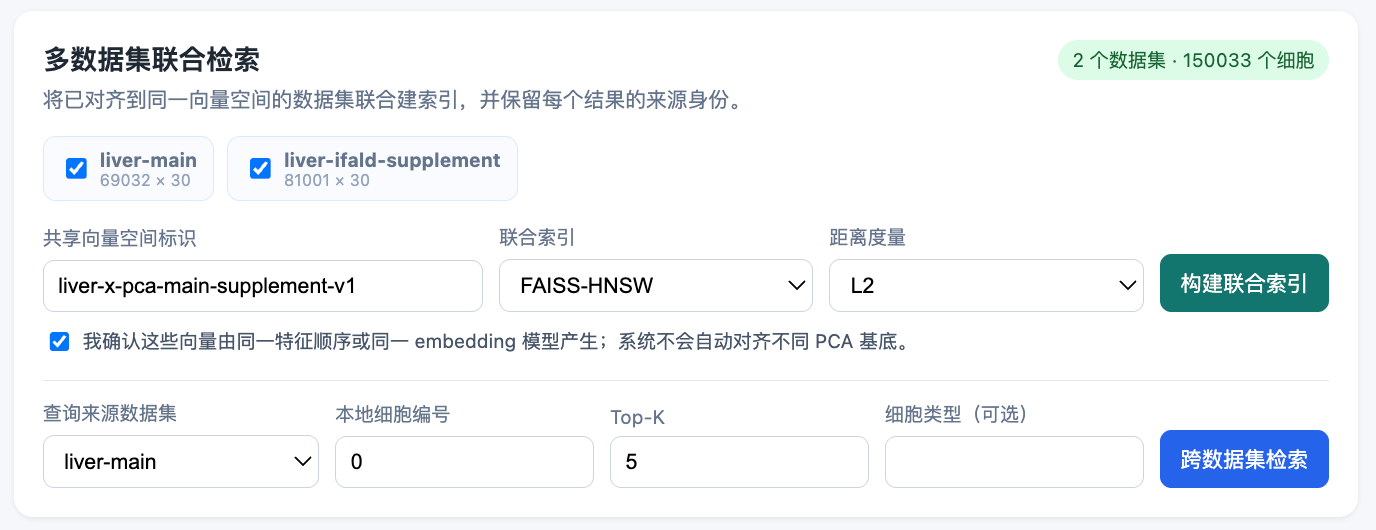
\includegraphics[width=0.88\textwidth]{24_federated_index_built.png}
  \caption{两个 H5AD 数据集的联合索引配置}
  \label{fig:federated-build}
\end{figure}

\begin{figure}[htbp]
  \centering
  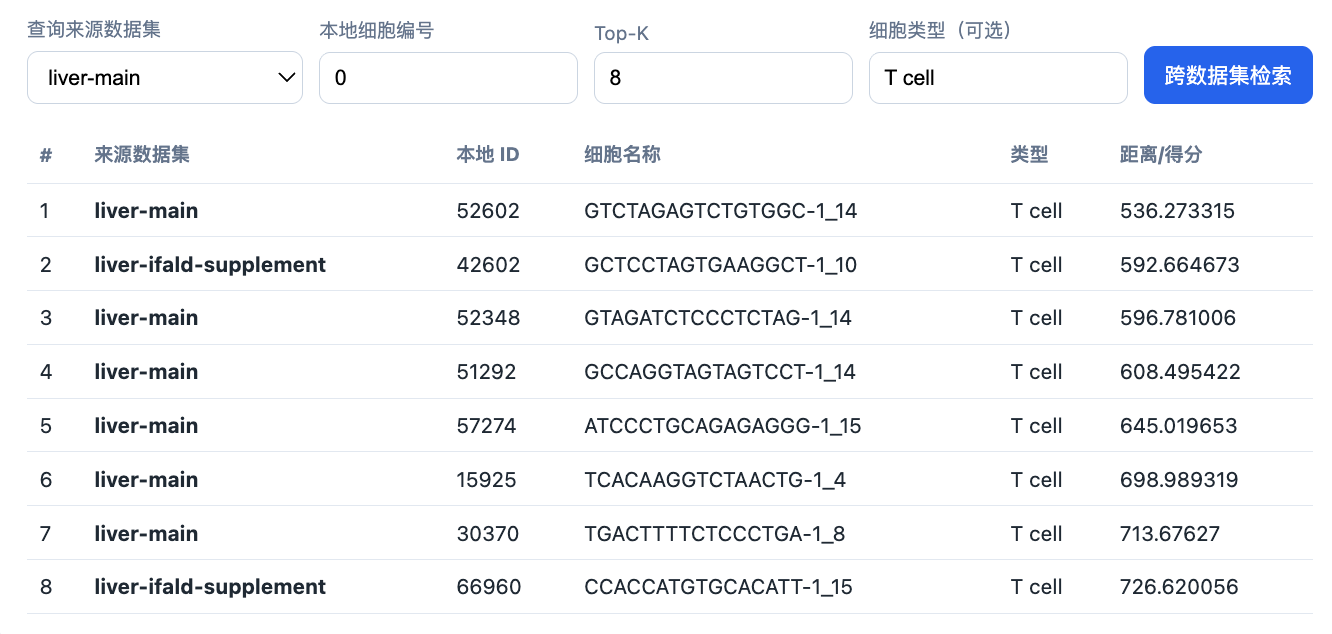
\includegraphics[width=0.88\textwidth]{25_federated_search_results.png}
  \caption{T cell 条件下的跨数据集 Top-8 检索结果}
  \label{fig:federated-results}
\end{figure}

该实验有两个必须说明的有效性边界。第一，\code{liver-main} 的 69,032 个细胞名全部包含在补充文件中，补充文件只新增 11,969 个 IFALD 细胞，简单拼接会重复大量细胞身份。第二，对 256 个重叠细胞抽样比较，两文件对应 \code{X\_pca} 的平均绝对差为 2.483，最大差为 67.438，说明“同为 30 维”不能证明 PCA 基底相同。因此本节只证明联合索引、条件过滤和来源追踪的工程能力，不据此解释跨数据集生物学相似性。严谨分析应先使用同一模型生成 embedding，或完成特征对齐和批次校正，并去除重复细胞。

\subsection{证据约束的自然语言助手}

助手先固定用户明确选择的数据集范围，再将问题解析为 \code{similar\_to\_cell}、\code{cell\_type\_representatives} 或 \code{dataset\_summary} 计划。服务端执行真实向量检索并生成数据集引用 [D\#] 和细胞证据引用 [E\#]；若配置外部生成模型，输出仍需通过引用白名单二次校验。未配置模型时返回确定性的本地证据摘要，不会伪装成 AI 成功。

\begin{figure}[htbp]
  \centering
  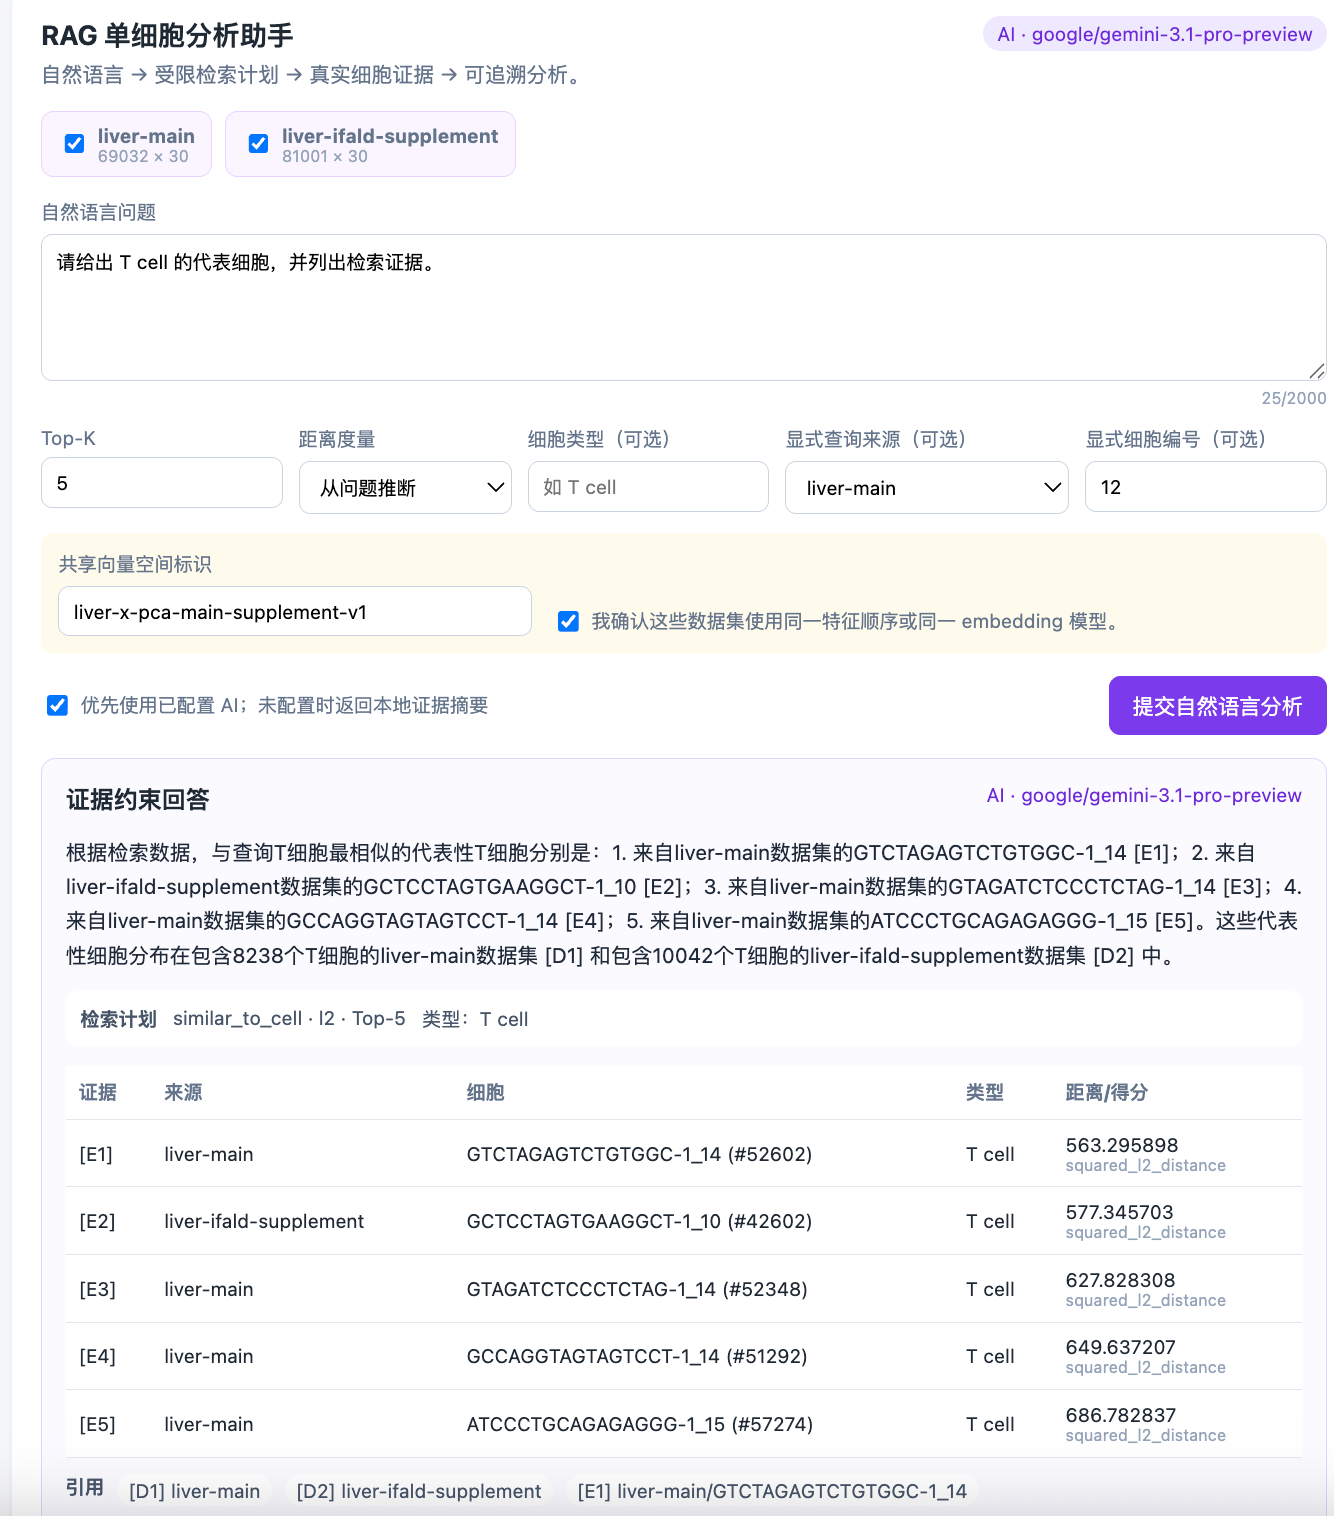
\includegraphics[width=0.69\textwidth]{27_rag_cell_type_representatives.png}
  \caption{RAG 助手的 T cell 代表细胞分析与可追溯证据链}
  \label{fig:rag}
\end{figure}

图\ref{fig:rag}展示自然语言问题、受限计划、跨数据集证据表和引用。系统不把原始向量发送给生成模型，也不保存问题与回答。输出只用于检索辅助；“代表细胞”表示靠近类型向量中心的结果，不等同于统计显著性、因果解释、诊断或临床建议。

\FloatBarrier
\section{系统测试}

\subsection{测试策略与覆盖范围}

后端使用 pytest 覆盖数据加载、索引、API、权限、持久化、历史、投影、联合检索和助手 provider 边界；前端使用 Vitest/jsdom 覆盖统一 API、认证门禁、资源管理、SVG 高亮、联合检索和证据 UI。文件生命周期测试使用临时目录和临时数据库，不保留上传副本、索引或日志。

\begin{table}[htbp]
  \centering
  \caption{主要功能与异常测试}
  \label{tab:function-tests}
  \begin{tabularx}{\textwidth}{p{0.19\textwidth}Y p{0.15\textwidth}}
    \toprule
    范围 & 代表性验证点 & 结果 \\
    \midrule
    认证与权限 & 注册/登录、过期或删除后令牌、管理员权限、生产配置保护 & 通过 \\
    数据格式 & H5AD/NPY/CSV、NaN/Inf、错误维度、对象数组、路径穿越 & 通过 \\
    检索正确性 & L2/Cosine/IP、Top-K 边界、自身排除、条件数量保证 & 通过 \\
    索引生命周期 & 全索引变体往返、指纹错配、损坏清单、失败原子性、级联删除 & 通过 \\
    评测 & 固定查询、有效 K、Recall、索引字节、PQ 成对摘要 & 通过 \\
    联合检索与 RAG & 共享空间确认、来源映射、失效、证据白名单、provider 失败 & 通过 \\
    前端交互 & 登录门禁、上传与索引管理、图上查询、历史与证据渲染 & 通过 \\
    \bottomrule
  \end{tabularx}
\end{table}

\subsection{质量门结果}

在 conda 的 \code{scann} 环境中执行以下命令：

\begin{lstlisting}
cd backend
ruff check .
ruff format --check .
PYTHONDONTWRITEBYTECODE=1 python -m pytest -q -p no:cacheprovider

cd ../frontend
npm run lint
NODE_OPTIONS=--no-experimental-webstorage npm test
npm run build
\end{lstlisting}

验证结果为：Ruff 检查通过，49 个 Python 文件格式符合要求，181 项后端测试全部通过；ESLint 通过，6 个前端测试文件中的 22 项测试全部通过，Vite 生产构建成功。截图 \code{35} 与 \code{36} 因终端提示符暴露本机用户/设备信息，且未完整显示所有质量门，故不进入报告；本节采用本次复核命令与文字结果。

\section{项目管理}

\subsection{版本管理与进度记录}

项目使用 Git 和 GitHub 管理，远程仓库为 \url{https://github.com/NKU-waiting/scANN}。提交按阶段组织，代表性记录包括：检索与评测正确性加固、认证安全、多数据集生命周期、索引持久化、历史与投影、图上查询、联合检索、PQ 重排、自然语言分析和完整演示文档。每个正式提交正文应包含 Changes、Verification 和 Scope，便于审查变更内容、验证步骤与影响范围。

\begin{table}[htbp]
  \centering
  \caption{项目阶段与主要交付物}
  \label{tab:project-stages}
  \begin{tabularx}{\textwidth}{p{0.15\textwidth}Y Y}
    \toprule
    阶段 & 核心任务 & 交付物 \\
    \midrule
    主链路 & 数据读取、Flat/ANN、Top-K、评测 & 后端服务、API、基础 UI 与测试 \\
    安全与资源 & JWT、上传校验、数据集和索引生命周期 & 元信息模型、指纹、原子发布与权限测试 \\
    交互完善 & 历史、UMAP/PCA、图上查询 & 前端组件、投影服务与回归测试 \\
    加分功能 & 联合检索、PQ 重排、RAG & 来源映射、理论保证、证据白名单 \\
    交付阶段 & 文档、截图、质量门、演示流程 & README、API/测试/用户文档与实验报告 \\
    \bottomrule
  \end{tabularx}
\end{table}

\subsection{人员分工与贡献度}

成员姓名、学号、角色和贡献度属于项目组外部确认信息，无法仅由代码仓库可靠推断，故不沿用模板中的个人信息，也不虚构比例。提交前请由全体成员确认并填写表\ref{tab:contribution}，贡献度总和应为 1。

\begin{table}[htbp]
  \centering
  \caption{成员分工与贡献度（提交前填写）}
  \label{tab:contribution}
  \begin{tabular}{p{0.18\textwidth}p{0.18\textwidth}p{0.42\textwidth}p{0.12\textwidth}}
    \toprule
    姓名 & 学号 & 负责内容 & 贡献度 \\
    \midrule
    \rule{0pt}{2.5ex} & & & \\
    \rule{0pt}{2.5ex} & & & \\
    \rule{0pt}{2.5ex} & & & \\
    \bottomrule
  \end{tabular}
\end{table}

\section{用户手册}

\subsection{安装与启动}

后端环境与启动命令如下：

\begin{lstlisting}
conda create -n scann python=3.12 -y
conda activate scann
cd backend
pip install -r requirements.txt
python run.py
\end{lstlisting}

前端在另一个终端启动：

\begin{lstlisting}
conda activate scann
cd frontend
npm ci
npm run dev
\end{lstlisting}

开发服务器默认由前端代理 \code{/api} 到后端。部署前应通过环境变量替换开发密钥和管理员密码，并配置允许的 CORS 来源；生产模式会拒绝默认安全配置。

\subsection{核心操作流程}

\begin{enumerate}
  \item 注册并登录；管理员登录后可查看额外管理区域。
  \item 在“数据集管理”上传 H5AD、NPY 或 CSV；H5AD 可指定 \code{X\_pca}、其他 \code{obsm} 字段或 \code{X}。
  \item 选择 Flat、IVF、HNSW、PQ 等索引和 L2/Cosine/IP 度量，构建索引。
  \item 按细胞编号或向量执行 Top-K 查询；需要时填写 \code{cell\_type} 条件。
  \item 查看结果表、距离/得分图、类型分布和 UMAP/PCA；可直接点击散点发起新查询。
  \item 保存当前索引；切换数据集或索引后，只加载与当前数据集指纹兼容的索引。
  \item 在评测面板选择多个索引，保持数据、度量、K 和查询数一致后比较 Recall、耗时和索引字节。
  \item 多数据集检索前必须确认所有表示来自同一特征顺序或 embedding 模型；不要只因维度相同就确认共享空间。
\end{enumerate}

\subsection{常见问题}

\begin{itemize}
  \item \textbf{H5AD 无法加载：}检查目标 \code{obsm} 字段、二维形状和 NaN/Inf；必要时显式选择 \code{X}。
  \item \textbf{索引无法加载：}确认数据集与索引清单绑定一致。文件或数据被修改后应重新构建。
  \item \textbf{条件结果少于 K：}候选数本身少于 K 时返回实际候选数，这是保证型条件检索的预期行为。
  \item \textbf{联合索引提示不兼容：}维度不同必须重新生成表示；维度相同仍需验证坐标空间和批次对齐。
  \item \textbf{RAG 显示本地证据模式：}这是未配置外部 provider 的正常降级，真实检索和引用仍然有效。
  \item \textbf{首次 UMAP 较慢：}首次调用可能触发 Numba 编译，后续会复用运行时缓存。
\end{itemize}

\section{总结、限制与未来工作}

本项目完成了课程要求的 Web 单细胞 ANN 检索主链路，并将数据、索引、查询、评测、可视化和权限组织为可演示、可测试的完整系统。实验表明 IVF 和 HNSW 在当前真实数据及参数下取得了较好的速度--召回权衡；PQ 显著降低索引字节，但基础排序损失较大；$4K$ 候选精确重排在索引字节不变的前提下稳定提高 Recall，验证了改进方向的有效性。

当前系统仍是单机课程演示：活动数据集、活动索引和联合索引为单进程共享状态，不支持多 worker 同步；SQLite 不适合高并发多租户；联合索引重启后需要重建；条件只支持 \code{cell\_type}；系统消费已有 embedding，不包含原始测序 QC；RAG 是受限检索辅助而不是开放域生物医学代理。现有两份真实数据还存在细胞重叠和 PCA 坐标不完全一致的问题。


\begin{thebibliography}{99}

\bibitem{anndata}
The scverse developers.
\newblock \emph{AnnData: An annotated data matrix}.
\newblock \url{https://anndata.readthedocs.io/en/stable/generated/anndata.AnnData.html}, 2026-07-12 访问.

\bibitem{faisswiki}
Meta AI Research.
\newblock \emph{Faiss Wiki: indexes and similarity search}.
\newblock \url{https://github.com/facebookresearch/faiss/wiki/Faiss-indexes}, 2026-07-12 访问.

\bibitem{hnsw}
Y. A. Malkov and D. A. Yashunin.
\newblock Efficient and robust approximate nearest neighbor search using Hierarchical Navigable Small World graphs.
\newblock \emph{IEEE Transactions on Pattern Analysis and Machine Intelligence}, 42(4):824--836, 2020.

\bibitem{pq}
H. Jegou, M. Douze, and C. Schmid.
\newblock Product quantization for nearest neighbor search.
\newblock \emph{IEEE Transactions on Pattern Analysis and Machine Intelligence}, 33(1):117--128, 2011.

\bibitem{umap}
L. McInnes, J. Healy, and J. Melville.
\newblock UMAP: Uniform Manifold Approximation and Projection for Dimension Reduction.
\newblock arXiv:1802.03426, 2018.

\bibitem{liverpaper}
R. D. Edgar, D. Nakib, D. Camat, et al.
\newblock Single-cell atlas of human pediatric liver reveals age-related hepatic gene signatures.
\newblock \emph{Hepatology Communications}, 9(11):e0813, 2025.
\newblock \url{https://doi.org/10.1097/HC9.0000000000000813}.

\bibitem{cellxgene}
CZ CELLxGENE Discover.
\newblock Liver single-cell collection.
\newblock \url{https://cellxgene.cziscience.com/collections/ff69f0ee-fef6-4895-9f48-6c64a68c8289}, 2026-07-12 访问.

\end{thebibliography}

\end{document}
